\chapter{Komplexit\"at von Algorithmen} 
In diesem Kapitel f\"uhren wir 
Rekurrenz-Gleichungen\footnote{
Rekurrenz-Gleichungen werden in der Literatur auch als \emph{Rekursions-Gleichungen} bezeichnet.}
ein und zeigen, wie diese in einfachen F\"allen gel\"ost werden k\"onnen.  Au{\ss}erdem stellen wir
die $O$-Notation vor.  Diese beiden Begriffe ben\"otigen wir, um die Laufzeit von
Algorithmen analysieren zu k\"onnen.  Die Algorithmen selber stehen in diesem Kapitel noch
im Hintergrund.

\section{Die Fibonacci-Zahlen}
Wir wollen \emph{Rekurrenz-Gleichungen} anhand eines eher spielerischen Beispiels
einf\"uhren.  Dazu betrachten wir eine Kaninchen-Farm, f\"ur die wir einen Gesch\"aftsplan
erstellen wollen.   Wir besch\"aftigen uns hier nur mit der Frage, wie sich eine
Kaninchen-Population entwickelt.  Wir gehen dabei von folgenden vereinfachenden Annahmen aus:
\begin{enumerate}
\item Jedes Kaninchen-Paar bringt jeden Monat ein neues Kaninchen-Paar zur Welt.
\item Kaninchen haben nach zwei Monaten zum ersten Mal Junge.
\item Kaninchen leben ewig.
\end{enumerate}
Wir nehmen nun an, wir h\"atten ein neugeborenes Kaninchen-Paar und stellen uns die Frage, wie
viele Kaninchen-Paare wir nach $n$ Monaten haben.  Bezeichnen wir die Zahl der
Kaninchen-Paare nach $n$ Monaten mit $k(n)$, so gilt:
\begin{enumerate}
\item $k(0) = 1$

      Wir starten mit einem neugeborenem Kaninchen-Paar.
\item $k(1) = 1$

      Kaninchen bekommen das erste Mal nach zwei Monaten Junge, also hat sich die Zahl
      der Kaninchen-Paare nach einem Monat noch nicht ver\"andert.
\item $k(2) = 1 + 1$

      Nach zwei Monaten bekommt unser Kaninchen-Paar zum ersten Mal Junge.
\item Allgemein gilt nach $n + 2$ Monaten: \\[0.1cm]
      \hspace*{1.3cm} 
      $k(n+2) = k(n+1) + k(n)$

      Alle Kaninchen-Paare, die zum Zeitpunkt $n$ schon da sind, bekommen zum Zeitpunkt
      $n+2$ Junge. Dies erkl\"art den Term $k(n)$.  Da wir zur Vereinfachung unserer
      Rechnung von genetisch manipulierten unsterblichen Kaninchen ausgehen, sind alle
      Kaninchen, die zum Zeitpunkt $n+1$ vorhanden sind, auch noch zum Zeitpunkt $n+2$
      vorhanden. Dies erkl\"art den Term $k(n+1)$. 
\end{enumerate}
Die Folge der Zahlen $\bigl(k(n)\bigr)_{n\in\mathbb{N}}$ hei{\ss}t Folge der \emph{Fibonacci-Zahlen}.  Das \Java-Programm in Abbildung
\ref{fig:fibonacci} auf Seite \pageref{fig:fibonacci} berechnet diese Zahlen.

\begin{figure}[!h]
  \centering
\begin{Verbatim}[ frame         = lines, 
                  framesep      = 0.3cm, 
                  labelposition = bottomline,
                  numbers       = left,
                  numbersep     = -0.2cm,
                  xleftmargin   = 0.8cm,
                  xrightmargin  = 0.8cm
                ]
    public class Fibonacci 
    {
        public static void main(String[] args) {
            for (int i = 0; i < 100; ++i) {
                int n = fibonacci(i);
                System.out.printf("fibonacci(%d) = %d\n", i, n);
            }
        }
        
        public static int fibonacci(int n) {
            if (n == 0) return 1;
            if (n == 1) return 1;
            return fibonacci(n - 1) + fibonacci(n - 2);
        }
    }
\end{Verbatim}
\vspace*{-0.3cm}
  \caption{Ein \textsl{Java}-Programm zur Berechnung der Fibonacci-Zahlen.}
  \label{fig:fibonacci}
\end{figure} 

Wenn wir dieses Programm laufen lassen, stellen wir fest, dass die Laufzeiten mit
wachsendem Parameter $n$ sehr schnell anwachsen.  Um dieses Ph\"anomen zu analysieren,
untersuchen wir exemplarisch, wie viele Additionen bei der Berechnung von
$\texttt{fibonacci}(n)$ f\"ur ein gegebenes $n \in \mathbb{N}$ ben\"otigt werden.  Bezeichnen wir
diese Zahl mit $a_n$, so finden wir:
\begin{enumerate}
\item $a_0 = 0$.
\item $a_1 = 0$.
\item $n \geq 2 \rightarrow a_n = a_{n-1} + a_{n-2} + 1$,

      denn in den rekursiven Aufrufen $\texttt{fibonacci}(n-1)$ und $\texttt{fibonacci}(n-2)$ haben wir 
      $a_{n-1}$ bzw.~$a_{n-2}$ Additionen und dazu kommt noch die Addition der Werte
      $\texttt{fibonacci}(n-1)$ und $\texttt{fibonacci}(n-2)$.
\end{enumerate}
Wir setzen in der  Gleichung $a_n = 1 + a_{n-1} + a_{n-2}$ f\"ur $n$ den Wert $i+2$ ein und
haben dann \\[0.1cm]
\hspace*{1.3cm} $a_{i+2} = a_{i+1} + a_i + 1$ \hspace*{\fill} $(1)$\\[0.1cm]
Eine solche Gleichung nennen wir eine \emph{lineare} \emph{inhomogene}
\emph{Rekur\-renz-Gleichung}.   Die dieser Gleichung zugeordnete \emph{homogene}
\emph{Rekurrenz-Gleichung} lautet \\[0.1cm]
\hspace*{1.3cm} $a_{i+2} = a_{i+1} + a_i$ \hspace*{\fill} $(2)$\\[0.1cm]
Wir l\"osen diese Gleichung mit folgendem Ansatz: \\[0.1cm]
\hspace*{1.3cm} $a_i = \lambda^i$. \\[0.1cm]
Einsetzen dieses Ansatzes in $(*)$ f\"uhrt auf die Gleichung 
\[ \lambda^{i+2} = \lambda^{i+1} + \lambda^i. \]
Wenn wir beide Seiten  dieser Gleichung durch $\lambda^i$ dividieren, erhalten wir die
quadratische Gleichung \\[0.1cm]
\hspace*{1.3cm} $\lambda^2 = \lambda + 1$, \\[0.1cm]
die wir mit Hilfe einer quadratischen Erg\"anzung l\"osen: \\[0.1cm]
\[\begin{array}{lcll}
  \lambda^2     & = & \lambda + 1                               & |\;- \lambda \\[0.1cm]
  \lambda^2 - 2 \cdot \frac{1}{2} \lambda & = & 1                   & |\;+ \frac{1}{4} \\[0.1cm]
  \lambda^2 - 2 \cdot \frac{1}{2} \lambda + \Big(\frac{1}{2}\Big)^2 & = &  \frac{5}{4} &  \\[0.1cm]
  \Big(\lambda -\frac{1}{2}\Big)^2 & = & \frac{5}{4}         & |\;\sqrt{\;\;} \\[0.1cm]
  \lambda -\frac{1}{2} & = & \pm\frac{\sqrt{5}}{2}           & | + \frac{1}{2} \\[0.1cm]
  \lambda_{1/2}  & = & \frac{1}{2} (1 \pm \sqrt{5}) & \\
 \end{array}
\]
Wir bemerken, dass jede Linear-Kombination der Form
\\[0.2cm]
\hspace*{1.3cm}
$a_n = \alpha \cdot \lambda_1^n + \beta \cdot \lambda_2^n$
\\[0.2cm]
eine L\"osung der homogenen Rekurrenz-Gleichung $(2)$ ist.
Wir bemerken weiter, dass f\"ur die L\"osungen $\lambda_1$ und $\lambda_2$ folgende Identit\"aten gelten:
\\[0.1cm]
\hspace*{1.3cm} 
$\lambda_1 - \lambda_2 = \sqrt{5}$ \quad und \quad $\lambda_1 + \lambda_2 = 1$. \hspace*{\fill} (3) \\[0.1cm]
Aus der letzen Gleichung folgt dann sofort \\[0.1cm]
\hspace*{1.3cm} $1 - \lambda_1 = \lambda_2$ \quad und \quad $1 - \lambda_2 = \lambda_1$ \hspace*{\fill} (4)  \\[0.1cm]
Um nun die urspr\"ungliche Rekurrenz-Gleichung (1) zu l\"osen, machen wir den Ansatz 
$a_i = c$.  Setzen wir diesen Ansatz in der Gleichung (1) ein, so erhalten wir die Gleichung \\[0.1cm]
\hspace*{1.3cm} $c = c + c + 1$, \\[0.1cm]
die die L\"osung $c = -1$ hat.  Diese L\"osung bezeichnen wir als eine \emph{spezielle L\"osumg}.
Die \emph{allgemeine L\"osung} der Rekurrenz-Gleichung (1) 
ergibt sich als Summe aus der L\"osung der homogenen Rekurrenz-Gleichung und der speziellen
L\"osung und lautet daher 
\[ a_i = \alpha \cdot \lambda_1^i + \beta \cdot \lambda_2^i - 1 \]
mit $\lambda_1 = \frac{1}{2} (1 + \sqrt{5})$ und $\lambda_2 = \frac{1}{2} (1 - \sqrt{5})$.
Die Koeffizienten $\alpha$ und $\beta$ sind jetzt so zu bestimmen, dass die
Anfangs-Bedingungen $a_0 = 0$ und $a_1 = 0$ erf\"ullt sind.  Das f\"uhrt auf folgendes
lineares Gleichungs-System: 
\[\begin{array}{lcl}
    0 & = & \alpha \cdot \lambda_1^0 + \beta \cdot \lambda_2^0 - 1 \\[0.1cm]
    0 & = & \alpha \cdot \lambda_1^1 + \beta \cdot \lambda_2^1 - 1 \\
  \end{array}
\]
Addieren wir bei beiden Gleichungen 1 und vereinfachen f\"ur $i=1,2$ die Potenzen $\lambda_i^0$ zu $1$ und
$\lambda_i^1$ zu $\lambda_i$, so erhalten wir:
\[\begin{array}{lcl}
    1 & = & \alpha + \beta \\[0.1cm]
    1 & = & \alpha \cdot \lambda_1 + \beta \cdot \lambda_2  \\
  \end{array}
\]
Die erste dieser beiden Gleichungen liefert die Beziehung $\alpha = 1 - \beta$.  Setzen
wir dies f\"ur $\alpha$ in der zweiten Gleichung ein, so erhalten wir 
\[
\begin{array}{clcl}
                      &  1 & = & (1 - \beta)\cdot  \lambda_1 + \beta \cdot \lambda_2 \\[0.1cm]
\Leftrightarrow\quad  &  1 & = & 
 \lambda_1  + \beta \cdot \bigl( \lambda_2 - \lambda_1\bigr) \\[0.1cm]
\Leftrightarrow\quad  &  1 - \lambda_1 & = & \beta \cdot \bigl(\lambda_2 - \lambda_1\bigr)  \\[0.1cm]
\Leftrightarrow\quad  &  \bruch{1 - \lambda_1}{\lambda_2 - \lambda_1} & = & \beta \\[0.1cm]
\end{array}
\]
Wegen $\alpha = 1 - \beta$ finden wir dann \\[0.1cm]
\hspace*{1.3cm} $\alpha = - \bruch{1 - \lambda_2}{\lambda_2 - \lambda_1}$. \\[0.1cm]
Verwenden  wir hier die Gleichungen (3) und (4), so finden wir \\[0.1cm]
\hspace*{1.3cm} 
$\alpha = \bruch{\lambda_1}{\sqrt{5}} $ \quad und \quad $\beta  = -\bruch{\lambda_2}{\sqrt{5}}$. \\[0.1cm]
Damit k\"onnen wir die Folge $(a_i)_i$ explizit angeben: \\[0.1cm]
\hspace*{1.3cm} 
$\displaystyle 
   a_i = \bruch{1}{\sqrt{5}} \cdot \left( \lambda_1^{i+1} - \lambda_2^{i+1} \right) - 1$ \\[0.1cm]
Wegen $\lambda_1\approx 1.61803$ und $\lambda_2 \approx - 0.61803$ dominiert der erste Term
der Summe und die Zahl der Additionen w\"achst exponentiell mit dem Faktor $\lambda_1$ an.
Dies erkl\"art das starke Anwachsen der Rechenzeit.
\vspace*{0.3cm}

\noindent
\textbf{Bemerkung}:  Die Zahl $\lambda_1$ wird auch als \emph{goldener Schnitt} bezeichnet
und spielt sowohl in der Geometrie als auch in der Kunst eine Rolle.

\noindent
Die Ursache der Ineffezienz der Berechnung der Fibonacci-Zahlen ist leicht zu sehen: Berechnen wir 
den Wert \texttt{fibonacci(5)} mit dem Programm aus Abbildung
\ref{fig:fibonacci}, so m\"ussen wir \texttt{fibonacci(4)} und \texttt{fibonacci(3)} berechnen.
Die Berechnung von \texttt{fibonacci(4)} erfordert ihrerseits die Berechnung von \texttt{fibonacci(3)} und \texttt{fibonacci(2)}. 
Dann berechnen wir \texttt{fibonacci(3)} aber zweimal!  
Abbildung \ref{fig:fibonacci.eps} zeigt den sogenannten \emph{Rekursions-Baum} f\"ur den
Aufruf von $\textsl{fibonacci}(5)$, der den oben dargestellten Zusammenhang graphisch verdeutlicht.

\begin{figure}[!ht]
  \centering
  \framebox{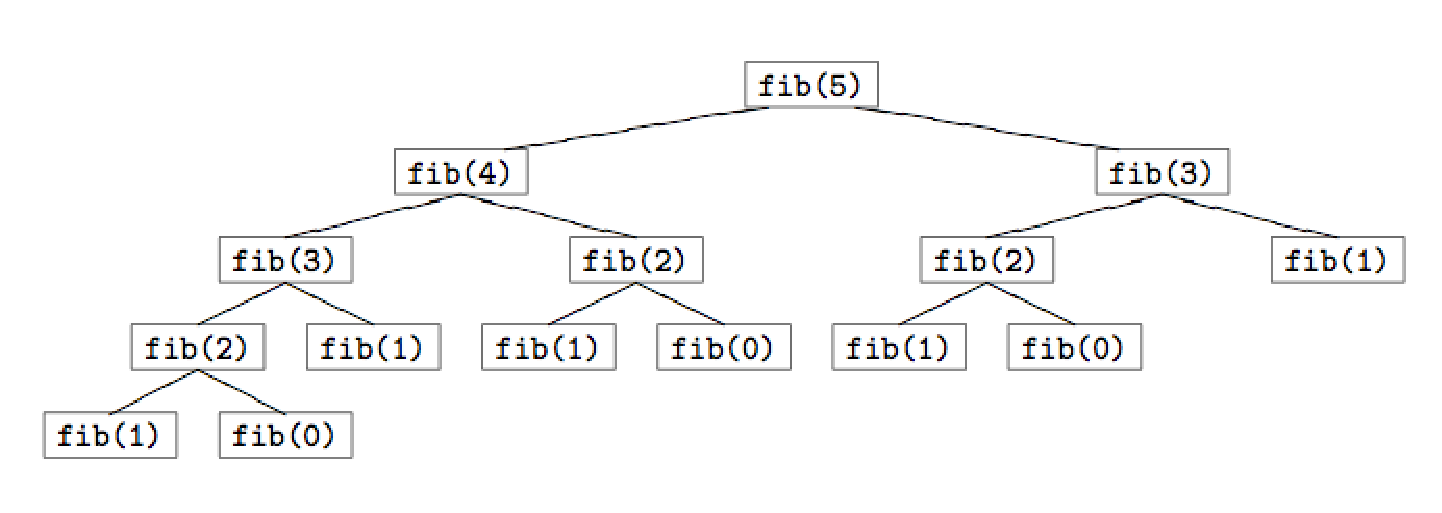
\epsfig{file=fibonacci.eps, scale=0.6}} 
  \caption{Rekursions-Baum f\"ur die Berechnung von $\textsl{fibonacci}(5)$.}
  \label{fig:fibonacci.eps}
\end{figure}


Wir k\"onnen eine effizientere Berechnung der Fibonacci-Zahlen implementieren, indem wir
uns die berechneten Werte merken.  Dazu k\"onnen wir in \Java\ ein Feld benutzen.
 Dies f\"uhrt zu dem in Abbildung \ref{fig:fibonacci-dynamic}
auf Seite \pageref{fig:fibonacci-dynamic} angegebenen Programm.
Da die Werte der Funktion \texttt{fibonacci}() exponentiell wachsen, reichen 32-Bit-Zahlen
nicht aus, um diese Werte darzustellen.  Wir verwenden daher die Klasse
\texttt{BigInteger}, mit der sich ganze Zahlen beliebiger Gr\"o{\ss}e darstellen lassen.
Da Felder in \Java\ genau wie in \texttt{C} mit 0 beginnend indiziert werden,
hat ein Feld, dessen oberster Index $n$ ist, insgesamt $n+1$ Elemente.  Wir legen daher in
Zeile 19 ein Feld von $n+1$ Elementen an.

\begin{figure}[!h]
  \centering
\begin{Verbatim}[ frame         = lines, 
                  framesep      = 0.3cm, 
                  labelposition = bottomline,
                  numbers       = left,
                  numbersep     = -0.2cm,
                  xleftmargin   = 0.8cm,
                  xrightmargin  = 0.8cm
                ]
    import java.math.*;
    
    public class FibonacciBig
    {
        public static void main(String[] args) 
        {
            for (int i = 0; i < 100; ++i) {
                BigInteger n = fibonacci(i);
                System.out.println("fib(" + i + ") = " + n);
            }
        }
        
        public static BigInteger fibonacci(int n) 
        {
            if (n <= 2) {
                return BigInteger.valueOf(1);
            }
            BigInteger[] mem = new BigInteger[n+1];
            mem[0] = BigInteger.valueOf(1);  // fibonacci(0) = 1
            mem[1] = BigInteger.valueOf(1);  // fibonacci(1) = 1
            for (int i = 0; i < n - 1; ++i) {
                mem[i + 2] = mem[i].add(mem[i + 1]);
            }
            return mem[n];
        }
    }
\end{Verbatim}
\vspace*{-0.3cm}
  \caption{Berechnung der Fibonacci-Zahlen mit Speicherung der Zwischenwerte.}
  \label{fig:fibonacci-dynamic}
\end{figure} 


\section{Lineare Rekurrenz-Gleichung \label{sec:lineare-RG}}
Wir waren bei der Analyse der Komplexit\"at des ersten Programms zur Berechnung der
Fibonacci-Zahlen auf die Gleichung \\[0.1cm]
\hspace*{1.3cm} $a_{i+2} = a_{i+1} + {a_i} + 1$ \quad f\"ur alle $i \in \mathbb{N}$ \\[0.1cm]
gesto{\ss}en. Gleichungen dieser Form treten bei der Analyse der Komplexit\"at rekursiver
Programme h\"aufig auf. Wir wollen uns daher in diesem Abschnitt n\"aher mit solchen
Gleichungen besch\"aftigen.

\begin{Definition}[Lineare homogene Rekurrenz-Gleichung] \hspace*{\fill} \\
{\em 
  Die \emph{lineare homogene Rekurrenz-Gleichung der Ordnung $k$ mit konstanten Koeffizienten} hat die Form
  \begin{equation}
    \label{eq:lhrg}
  a_{n+k} = c_{k-1} \cdot a_{n+k-1} + c_{k-2} \cdot a_{n+k-2} + \cdots + c_1 \cdot a_{n+1} + c_0 \cdot a_{n}
     \quad \mbox{f\"ur alle $n \in \N$}. 
  \end{equation}
     In Summen-Schreibweise kann diese Gleichung kompakter als 
     \\[0.1cm]
     \hspace*{1.3cm}
     $a_{n+k} = \sum\limits_{i=0}^{k-1} c_i \cdot a_{n+i}$ \quad f\"ur alle $n \in \mathbb{N}$
     \\[0.1cm]
     geschreiben werden.
     Zus\"atzlich werden \emph{Anfangs-Bedingungen}  
      \\[0.1cm]
      \hspace*{1.3cm}      
      $a_0 = d_0, \cdots, a_{k-1} = d_{k-1}$ 
      \\[0.1cm]
      f\"ur die Folge $\folge{a_n}$ vorgegeben.    
    \hspace*{\fill} $\Box$
}
\end{Definition}
Durch eine lineare homogene Rekurrenz-Gleichung wird die Folge $(a_n)_{n\in\mathbb{N}}$
eindeutig bestimmt: Die Werte $a_n$ f\"ur $n < k$ sind durch die Anfangs-Bedingungen gegeben und
alle weiteren Werte k\"onnen dann durch die Rekurrenz-Gleichung (\ref{eq:lhrg}) bestimmt werden.
Noch  etwas zur Nomenklatur:
\begin{enumerate}
\item Die Rekurrenz-Gleichung (\ref{eq:lhrg}) hei{\ss}t \emph{linear}, weil die Glieder der Folge $(a_n)_n$ nur
      linear in der Gleichung (\ref{eq:lhrg}) auftreten.  Ein Beispiel f\"ur eine
      Rekurrenz-Gleichung, die nicht linear ist, w\"are \\[0.1cm]
      \hspace*{1.3cm} $a_{n+1} = a_n^2$ \quad f\"ur alle $n \in \mathbb{N}$. \\[0.1cm]
      Nicht-lineare Rekurrenz-Gleichungen sind nur in Spezialf\"allen geschlossen l\"osbar.
\item Die Rekurrenz-Gleichung (\ref{eq:lhrg}) hei{\ss}t \emph{homogen}, weil auf der rechten Seite
      dieser Gleichung kein konstantes Glied mehr auftritt.  Ein Beispiel f\"ur eine
      Gleichung, die nicht homogen ist (wir sprechen auch von \emph{inhomogenen}
      Rekurrenz-Gleichungen), w\"are \\[0.1cm]
      \hspace*{1.3cm} $a_{n+2} = a_{n+1} + a_n + 1$ \quad f\"ur alle $n \in \mathbb{N}$. \\[0.1cm]
      Mit inhomogenen Rekurrenz-Gleichungen werden wir uns sp\"ater noch besch\"aftigen.
\item Die Rekurrenz-Gleichung (\ref{eq:lhrg}) hat \emph{konstante Koeffizienten}, weil die
      Werte $c_i$ Konstanten sind, die nicht von dem Index $n$ abh\"angen.  Ein Beispiel f\"ur
      eine Rekurrenz-Gleichung, die keine konstanten Koeffizienten hat, ist \\[0.1cm]
      \hspace*{1.3cm} $a_{n+1} = n\cdot a_n$ \quad f\"ur alle $n \in \mathbb{N}$. \\[0.1cm]
      Solche Rekurrenz-Gleichungen k\"onnen in vielen F\"allen auf Rekurrenz-Gleichungen mit
      konstanten Koeffizienten zur\"uck gef\"uhrt werden.  Wir werden das sp\"ater noch im
      Detail besprechen.
\end{enumerate}
Wie l\"osen wir eine lineare homogene Rekurrenz-Gleichung?  Wir versuchen zun\"achst den Ansatz\\[0.1cm]
\hspace*{1.3cm}  $a_n = \lambda^n$ \quad f\"ur alle $n \in \mathbb{N}$. \\[0.1cm]
Einsetzen dieses Ansatzes in (\ref{eq:lhrg}) f\"uhrt auf die Gleichung \\[0.1cm]
\hspace*{1.3cm}
$\lambda^{n+k} = \sum\limits_{i=0}^{k-1} c_i \cdot \lambda^{n+i}$
\\[0.1cm]
Dividieren wir diese Gleichung durch $\lambda^n$, so haben wir: \\[0.1cm]
\hspace*{1.3cm} $\lambda^{k} = \sum\limits_{i=0}^{k-1} c_i \cdot \lambda^{i}$  
\\[0.1cm]
Das Polynom \\[0.1cm]
\hspace*{1.3cm} 
$\chi(x) = x^{k} - \sum\limits_{i=0}^{k-1} c_i \cdot x^{i}$  
\\[0.1cm]
 hei{\ss}t \emph{charakteristisches Polynom} der Rekurrenz-Gleichung (\ref{eq:lhrg}).
Wir betrachten zun\"achst den Fall, dass das charakteristische  Polynom  $k$  verschiedene
Nullstellen hat.  In diesem Fall sagen, dass die Rekurrenz-Gleichung (\ref{eq:lhrg}) 
\emph{nicht entartet} ist.
Bezeichnen wir diese Nullstellen mit \\[0.1cm]
\hspace*{1.3cm}  $\lambda_1$, $\lambda_2$, $\cdots$, $\lambda_k$, \\[0.1cm]
so  gilt f\"ur alle $j = 1,\cdots, k$ \\[0.1cm]
\hspace*{1.3cm} 
$\lambda_j^{n+k} = \sum\limits_{i=0}^{k-1} c_i \cdot \lambda_j^{n+i}$.
\\[0.1cm]
Damit ist die Folge  
\[\bigl(\lambda_j^n)_{n\in\mathbb{N}}\]
f\"ur alle $j=1,\cdots,k$ eine L\"osung der Rekurrenz-Gleichung (\ref{eq:lhrg}).
Au{\ss}erdem ist auch jede Linear-Kombination dieser L\"osungen eine L\"osung von (\ref{eq:lhrg}):
Definieren wir die Folge $a_n$ durch \\[0.1cm]
\hspace*{1.3cm} $a_n = \alpha_1 \lambda_1^n + \cdots + \alpha_k \lambda_k^n$ \quad f\"ur alle $n \in \mathbb{N}$ \\[0.1cm]
mit beliebigen Koeffizienten $\alpha_i \in \R$, so erf\"ullt auch die Folge
$(a_n)_n$ die Gleichung (\ref{eq:lhrg}).  Die oben definierte Folge $(a_n)_n$ bezeichnen wir als
die  \emph{allgemeine L\"osung} der Rekurrenz-Gleichung (\ref{eq:lhrg}): \\[0.1cm]
Die Koeffizienten $\alpha_1$ bis $\alpha_k$ m\"ussen wir nun so w\"ahlen, dass die
Anfangs-Bedingungen 
\\[0.2cm]
\hspace*{1.3cm}
$a_0 = d_0$, $\cdots$, $a_{k-1} = d_{k-1}$
\\[0.2cm]
erf\"ullt sind.  Das liefert ein lineares Gleichungs-System f\"ur die Koeffizienten $\alpha_1$, $\cdots$, $\alpha_k$:
\[
\begin{array}{lcl}
  d_0     & = & \lambda_1^0 \cdot \alpha_1 + \cdots +   \lambda_k^0 \cdot \alpha_k \\[0.1cm]
  d_1     & = & \lambda_1^1 \cdot \alpha_1 + \cdots +   \lambda_k^1 \cdot \alpha_k \\[0.1cm]
  \vdots  &   & \vdots                                                   \\[0.1cm]
  d_{k-1} & = & \lambda_1^{k-1} \cdot \alpha_1 + \cdots +   \lambda_{k}^{k-1} \cdot \alpha_k \\[0.1cm]
\end{array}
\]
Hier sind die Werte $\lambda_i$  die Nullstellen des charakteristischen Polynoms.  
Die Matrix $V$, die diesem Gleichungs-System
zugeordnet ist, lautet: 
\[
V = \left(
\begin{array}{lcl}
  \lambda_1^0  & \cdots &   \lambda_k^0 \\[0.1cm]
  \lambda_1^1  & \cdots &   \lambda_k^1 \\[0.1cm]
  \vdots         &         & \vdots \\[0.1cm]
  \lambda_1^{k-1} & \cdots &   \lambda_{k}^{k-1} \\[0.1cm]
\end{array}\right)
\]
Diese Matrix ist in der Mathematik als \emph{Vandermonde}'sche Matrix bekannt.  F\"ur die
Determinate dieser Matrix gilt \\[0.1cm]
\hspace*{1.3cm} $\det(V) = \prod\limits_{1 \leq i < j \leq k} (\lambda_i - \lambda_j)$. \\[0.1cm]
Sind die Nullstellen $\lambda_i$ f\"ur $i=1,\cdots,k$ paarweise verschieden, so ist jeder
der Faktoren $(\lambda_i - \lambda_j)$ von 0 verschieden und damit ist auch das Produkt
von 0 verschieden.  Daraus folgt, das das zugeh\"orige lineare Gleichungs-System eindeutig
l\"osbar ist.  Mit der L\"osung dieses Gleichungs-Systems
 haben wir dann die L\"osung der Rekurrenz-Gleichung (\ref{eq:lhrg}) gefunden.
\vspace*{0.1cm}

\noindent
\textbf{Beispiel}:  Wie demonstrieren das Verfahren an einem Beispiel: Wie betrachten die
Rekurrenz-Gleichung \\[0.1cm]
\hspace*{1.3cm} $F_{n+2} = F_{n+1} + F_{n}$ \quad f\"ur alle $n \in \mathbb{N}$  \\[0.1cm]
mit den Anfangs-Bedingungen $F_0 = 0$ und $F_1 = 1$.  Die L\"osung dieser
Rekurrenz-Gleichung sind \"ubrigens gerade die Fibonacci-Zahlen.
Das \emph{charakteristische Polynom} dieser Rekurrenz-Gleichung lautet: \\[0.1cm]
\hspace*{1.3cm} $\chi(x) = x^2 - x - 1$.  \\[0.1cm]
Das f\"uhrt auf die quadratische Gleichung \\[0.1cm]
\hspace*{1.3cm} $x^2 -x - 1 = 0$ \\[0.1cm]
Wir haben eben schon gesehen, dass diese quadratische Gleichung die L\"osung \\[0.1cm]
\hspace*{1.3cm}
 $ x_{1/2} = \frac{1}{2} \cdot (1 \pm \sqrt{5})$ 
\\[0.1cm]
hat.  Wir definieren \\[0.1cm]
\hspace*{1.3cm} 
$\lambda_1 = \frac{1}{2} \cdot (1 + \sqrt{5})$ \quad und  \quad 
$\lambda_2 = \frac{1}{2} \cdot (1 - \sqrt{5})$. \\[0.1cm]
Damit lautet die \emph{allgemeine L\"osung} der betrachteten Rekurrenz-Gleichung \\[0.1cm]
\hspace*{1.3cm}  $F_n = \alpha_1 \cdot \lambda_1^n  + \alpha_2 \cdot \lambda_2^n$ \quad f\"ur alle $n \in \mathbb{N}$. \\[0.1cm]
Setzen wir hier die Anfangs-Bedingungen ein, so erhalten wir
\[
\begin{array}{lcl}
    0 & = & \lambda_1^0 \cdot \alpha_1 + \lambda_2^0   \cdot \alpha_2 \\[0.1cm]
    1 & = & \lambda_1^1 \cdot \alpha_1 + \lambda_2^{1} \cdot \alpha_2 
\end{array}
\]
Dies ist ein lineares Gleichungs-System in den Unbekannten $\alpha_1$ und
$\alpha_2$. Vereinfachung f\"uhrt auf 
\[
\begin{array}{lcl}
    0 & = & \alpha_1 + \alpha_2 \\[0.1cm]
    1 & = & \lambda_1 \cdot \alpha_1 + \lambda_2 \cdot \alpha_2 
\end{array}
\]
Die erste dieser beiden Gleichungen l\"osen wir nach $\alpha_2$ auf und finden  $\alpha_2 = - \alpha_1$.
Diesen Wert setzen wir in der zweiten Gleichung ein.  Das f\"uhrt auf
\[
\begin{array}{lrcl}
                 & 1 & = & \lambda_1 \cdot \alpha_1 - \lambda_2 \cdot \alpha_1 \\
 \Leftrightarrow & 1 & = & (\lambda_1 - \lambda_2) \cdot \alpha_1 \\
 \Leftrightarrow & \bruch{1}{\lambda_1 - \lambda_2} & = & \alpha_1 \\
\end{array}
\]
Setzen wir diesen Wert in der Gleichung $\alpha_2 = - \alpha_1$ ein, so erhalten wir \\[0.1cm]
\hspace*{1.3cm} 
  $\alpha_2 = \bruch{- 1}{\lambda_1 - \lambda_2}$.
\\[0.1cm]
Setzen wir die  Werte f\"ur $\lambda_1$ und $\lambda_2$ ein, so finden wir:  \\[0.1cm]
\hspace*{1.3cm} 
$\alpha_1 = \bruch{1}{\sqrt{5}}$ \quad und \quad $\alpha_2 = - \bruch{1}{\sqrt{5}}$.
\\[0.1cm]
Die L\"osung der Rekurrenz-Gleichung \\[0.1cm]
\hspace*{1.3cm} $F_{n+2} = F_{n+1} + F_{n}$ \quad f\"ur alle $n \in \mathbb{N}$ \\[0.1cm]
mit den Anfangs-Bedingungen $F_0 = 1$ und $F_1 = 1$   lautet also 
\\[0.1cm]
\hspace*{1.3cm} 
$F_n = \bruch{1}{\sqrt{5}}\cdot \left( \lambda_1^{n} - \lambda_2^{n} \right)$ 
\quad f\"ur alle $n \in \mathbb{N}$.  
\\[0.1cm]
Damit haben wir eine geschlossene Formel zur Berechnung der Fibonacci-Zahlen
gefunden.  Diese Formel zeigt uns, dass die Fibonacci-Zahlen selbst exponentiell anwachsen.
Wir werden diese L\"osung bei der Analyse des Euklidischen-Algorithmus ben\"otigen.

\vspace*{0.2cm}
\noindent
\textbf{Aufgabe}:  L\"osen Sie die Rekurrenz-Gleichung 
$a_{n+2} = \bruch{3}{2} \cdot a_{n+1} - \bruch{1}{2}\cdot a_n$ mit
den Anfangs-Bedingungen $a_0 = 3$ und $a_1 = \bruch{5}{2}$.

%\noindent
%\textbf{L\"osung}: $a_n = 2 + \left(\frac{1}{2}\right)^n$.

\subsection{Entartete Rekurrenz-Gleichungen}
Wir hatten oben zun\"achst den Fall betrachtet, dass das charakteristische Polynom der
Rekurrenz-Gleichung (\ref{eq:lhrg}) insgesamt $k$ verschiedene Nullstellen hat.   Dies muss
keineswegs immer der Fall sein.  Wir betrachten die Rekurrenz-Gleichung 
\begin{equation}
  \label{eq:erg}
  a_{n+2} = 4 \cdot a_{n+1} - 4 \cdot a_n \quad \mbox{f\"ur alle $n \in \mathbb{N}$} 
\end{equation}
 mit den Anfangs-Bedingungen $a_0 = 1$, $a_1 = 4$.  Das charakteristische Polynom lautet \\[0.1cm]
\hspace*{1.3cm} $\chi(x) = x^2 - 4 \cdot x + 4 = (x - 2)^2$ \\[0.1cm]
und hat offensichtlich nur eine Nullstelle bei $x = 2$.   Eine L\"osung der
Rekurrenz-Gleichung (\ref{eq:erg}) lautet daher \\[0.1cm]
\hspace*{1.3cm} $a_n = 2^n$ \quad f\"ur alle $n \in \mathbb{N}$. \\[0.1cm]
Eine weitere L\"osung ist \\[0.1cm]
\hspace*{1.3cm} $a_n = n \cdot 2^n$ \quad f\"ur alle $n \in \mathbb{N}$.  \\[0.1cm]
Wir verifizieren dies durch Einsetzen: 
\[
\begin{array}{llcll}
 & (n+2) \cdot 2^{n+2} & = & 4 \cdot (n+1) \cdot 2^{n+1} - 4 \cdot n \cdot 2^n & \mid\; \div 2^n \\
\Leftrightarrow & 
   (n+2) \cdot 2^{2} & = & 4 \cdot (n+1) \cdot 2^{1} - 4 \cdot n  &  \mid\; \div 4 \\
\Leftrightarrow & n + 2 & = & (n + 1) \cdot 2 -  n  &  \\
\Leftrightarrow & n + 2 & = & 2 \cdot n + 2 -  n   \\
\Leftrightarrow & n + 2 & = & n + 2    \\
\end{array}
\]
Die allgemeine L\"osung der Rekurrenz-Gleichung finden wir durch Linear-Kombination der
beiden L\"osungen: \\[0.1cm]
\hspace*{1.3cm} $a_n = \alpha \cdot 2^n + \beta \cdot n \cdot 2^n$ \quad f\"ur alle $n \in \mathbb{N}$. \\[0.1cm]
Setzen wir hier die Anfangs-Bedingungen $a_0 = 1$ und $a_2 = 4$ ein, so erhalten wir:
\[
\left\{
\begin{array}{lcl}
  1 & = & \alpha \cdot 2^0 + \beta \cdot 0 \cdot 2^0 \\
  4 & = & \alpha \cdot 2^1 + \beta \cdot 1 \cdot 2^1 \\
\end{array}
\right\} \quad\Leftrightarrow\quad \left\{
\begin{array}{lcl}
  1 & = & \alpha \\
  4 & = & \alpha \cdot 2 + \beta \cdot 2 \\
\end{array}
\right\}\]
Die L\"osung lautet offenbar $\alpha = 1$ und $\beta = 1$.  Damit lautet die L\"osung der
Rekurrenz-Gleichung (\ref{eq:erg}) mit den Anfangs-Bedingungen $a_0 = 1$ und $a_2 = 4$ \\[0.1cm]
\hspace*{1.3cm} $a_n = 2^n + n \cdot 2^n = (n+1) \cdot 2^n$ \quad f\"ur alle $n \in \mathbb{N}$.  \\[0.1cm]
Im allgemeinen nennen wir die Rekurrenz-Gleichung \\[0.1cm]
\hspace*{1.3cm} $a_{n+k} = \sum\limits_{i=0}^{k-1} c_{i} \cdot a_{n+i}$ \\[0.1cm]
\emph{entartet}, wenn das charakteristische Polynom \\[0.1cm]
\hspace*{1.3cm} $\chi(x) = x^k - \sum\limits_{i=0}^{k-1} c_{i} \cdot x^{i}$  \\[0.1cm]
weniger als $k$ verschiedene Nullstellen hat.  Dann l\"asst sich folgendes
zeigen:  Hat das charakteristische Polynom $\chi(x)$ eine $r$-fache Nullstelle
$\lambda$, gilt also \\[0.1cm]
\hspace*{1.3cm} $\chi(x) = (x - \lambda)^r \cdot \phi(x)$ \\[0.1cm]
mit einem geeigneten Polynom $\phi(x)$, so sind die Folgen
\begin{enumerate}
\item $(\lambda^n)_{n\in\mathbb{N}}$
\item $(n\cdot\lambda^n)_{n\in\mathbb{N}}$
\item $(n^2\cdot\lambda^n)_{n\in\mathbb{N}}$
\item $\vdots$
\item $(n^{r-1}\cdot\lambda^n)_{n\in\mathbb{N}}$
\end{enumerate}
L\"osungen der Rekurrenz-Gleichung (\ref{eq:erg}).  Durch eine geeignete Linear-Kombination dieser
L\"osungen zusammen mit den L\"osungen, die sich aus den Nullstellen des Polynoms $\phi$
ergeben, l\"asst sich dann immer eine L\"osung finden, die auch den Anfangs-Bedingungen gen\"ugt.
\vspace*{0.3cm}

\noindent
\textbf{Aufgabe}: L\"osen Sie die Rekurrenz-Gleichung \\[0.1cm]
\hspace*{1.3cm} $a_{n+3} = a_{n+2} + a_{n+1} - a_n$ \\[0.1cm]
f\"ur die Anfangs-Bedingungen $a_0 = 0$, $a_1 = 3$, $a_2 = 2$.

%\noindent
%\textbf{L\"osung}: allg. $a_n = \alpha + n \cdot \beta + \gamma \cdot (-1)^n$. 
%Anfangs-Bedingungen: $a_n = 1 + n - (-1)^n$.

\subsection{Inhomogene Rekurrenz-Gleichungen}    
\begin{Definition}[Lineare inhomogene Rekurrenz-Gleichung]
{\em Die \emph{lineare \underline{inhomo}g\underline{ene} Rekur\-renz-Gleichung der Ordnung
$k$ mit konstanten Koeffizienten und konstanter Inhomogenit\"at} hat die Form 
\begin{equation}
  \label{eq:lihrg}
     a_{n+k} = \sum\limits_{i=0}^{k-1} c_{i} \cdot a_{n+i} + c_{-1}  
\end{equation}
     mit den Anfangs-Bedingungen $a_0 = d_0$, $\cdots$, $a_{k-1} = d_{k-1}$. 
     Dabei gilt f\"ur die Koeffizienten \\[0.1cm]
     \hspace*{1.3cm} $c_i \in \R$ \quad f\"ur alle $i = -1, 0,\cdots, k-1$. \\[0.1cm]
     F\"ur die  \emph{Anfangs-Bedingungen} $d_0, \cdots, d_{k-1}$ gilt ebenfalls \\[0.1cm]
     \hspace*{1.3cm} $d_i \in \R$ \quad f\"ur alle $i = 0,\cdots, k-1$. \\[0.1cm]
     Die Konstante $c_{-1}$ bezeichnen wir als die \emph{Inhomogenit\"at}. 
     \hspace*{\fill} $\Box$
}
\end{Definition}

Wie l\"asst sich die inhomogene Rekurrenz-Gleichung (\ref{eq:lihrg}) l\"osen? Wir zeigen
zun\"achst, wie sich eine \emph{spezielle L\"osung} der Rekurrenz-Gleichung (\ref{eq:lihrg})
finden l\"asst.  Dazu betrachten wir das charakteristische Polynom \\[0.1cm]
\hspace*{1.3cm} 
$\chi(x) = x^k - \sum\limits_{i=0}^{k-1} c_{i} \cdot x^i$
\\[0.1cm]
und definieren die \emph{Spur} $\mathtt{sp}(\chi)$ wie folgt: \\[0.1cm]
\hspace*{1.3cm} 
$\mathtt{sp}(\chi) := \chi(1) = 1 - \sum\limits_{i=0}^{k-1} c_{i}$. \\[0.1cm]
Es k\"onnen zwei F\"alle auftreten, $\mathtt{sp}(\chi) \not= 0$ und
$\mathtt{sp}(\chi) = 0$.
Wir betrachten die beiden F\"alle getrennt.
\begin{enumerate}
\item $\mathtt{sp}(\chi) \not= 0$.

      Dann erhalten wir eine spezielle L\"osung von (\ref{eq:lihrg}) durch den Ansatz \\[0.1cm]
      \hspace*{1.3cm} $a_n = \delta$ \quad f\"ur alle $n \in \mathbb{N}$. \\[0.1cm]
      Den Wert von $\delta$ bestimmen wir durch Einsetzen, es muss f\"ur alle $n\in \mathbb{N}$ gelten: \\[0.1cm]
      \hspace*{1.3cm} 
      $\delta = \sum\limits_{i=0}^{k-1} c_{i} \cdot \delta + c_{-1}$.
      \\[0.1cm]
      Daraus ergibt sich \\[0.1cm]
      \hspace*{1.3cm} 
      $\delta \cdot \left(1 - \sum\limits_{i=0}^{k-1} c_{i} \right) =  c_{-1}$. \\[0.1cm]
      Das ist aber nichts anderes als \\[0.1cm]
      \hspace*{1.3cm} $\delta \cdot \mathtt{sp}(\chi) = c_{-1}$ \\[0.1cm]
      und damit lautet eine spezielle L\"osung von (\ref{eq:lihrg}) \\[0.1cm]
      \hspace*{1.3cm} $a_n = \delta = \bruch{c_{-1}}{\mathtt{sp}(\chi)}$.
      \\[0.1cm]
      Jetzt sehen wir auch, warum die Voraussetzung $\mathtt{sp}(\chi) \not= 0$
      wichtig ist, denn anderfalls w\"are der Quotient
      $\bruch{c_{-1}}{\mathtt{sp}(\chi)}$ undefiniert.
\item $\mathtt{sp}(\chi) = 0$.

      In diesem Fall versuchen wir, eine spezielle L\"osung von (\ref{eq:lihrg}) durch den
      Ansatz \\[0.1cm]
      \hspace*{1.3cm} $a_n = \varepsilon \cdot n $ \\[0.1cm]
      zu finden.  Den Wert $\varepsilon$ erhalten wir durch Einsetzen, es muss f\"ur 
      alle $n\in\mathbb{N}$ gelten: \\[0.1cm]
      \hspace*{1.3cm} 
      $\varepsilon \cdot (n + k) = \sum\limits_{i=0}^{k-1} c_{i} \cdot \varepsilon \cdot (n + i) + c_{-1}$  
      \\[0.1cm]
      Dies formen wir wie folgt um:
      \[
        \varepsilon \cdot n + \varepsilon \cdot k = 
        \varepsilon \cdot n \cdot \sum\limits_{i=0}^{k-1} c_{i} +
        \varepsilon \cdot \sum\limits_{i=0}^{k-1} i \cdot c_{i} + c_{-1} 
      \]
      Aus  $\mathtt{sp}(\chi) = 0$ folgt $1  =  \sum\limits_{i=0}^{k-1} c_i$
      und damit gilt \\[0.1cm]
      \hspace*{1.3cm} 
      $\varepsilon \cdot n = \varepsilon \cdot n \cdot \sum\limits_{i=0}^{k-1} c_{i}$.
      \\[0.1cm]
      Daher vereinfacht sich die obige Gleichung zu 
      \[
      \begin{array}{ll}
      & \varepsilon \cdot k = \varepsilon \cdot \sum\limits_{i=0}^{k-1} i \cdot c_{i} + c_{-1} \\[0.4cm]
      \Leftrightarrow\quad 
      & \varepsilon \cdot \left(k - \sum\limits_{i=0}^{k-1} i \cdot c_{i}\right) = c_{-1} 
      \\[0.5cm]
      \Leftrightarrow\quad 
      & \varepsilon = \frac{\displaystyle c_{-1}}{\displaystyle \; k - \sum\limits_{i=0}^{k-1} i \cdot c_{i}\;} 
      \end{array}
      \]
      Wenn wir genau hin schauen, dann sehen wir, dass der Wert im Nenner nicht anderes ist
      als der Wert der Ableitung des charakteristischen Polynoms an der Stelle 1, denn es gilt: \\[0.1cm]
      \hspace*{1.3cm} 
      $\chi'(x) =\bruch{d\,\chi(x)}{dx} = k \cdot x^{k-1} - \sum\limits_{i=0}^{k-1} c_{i}\cdot i \cdot x^{i-1}$
      \\[0.1cm]
      Setzen wir hier f\"ur $x$ den Wert $1$ ein, so finden wir \\[0.1cm]
      \hspace*{1.3cm} 
      $\chi'(1) = k - \sum\limits_{i=0}^{k-1} c_{i}\cdot i$. 
      \\[0.1cm]
      Insgesamt haben wir damit also die folgende spezielle L\"osung $(a_n)_{n\in\mathbb{N}}$
      der Gleichung (\ref{eq:lihrg}) gefunden: \\[0.1cm]
      \hspace*{1.3cm} $a_n = \bruch{c_{-1}}{\;\chi'(1)\;}\cdot n$.

      Wir haben oben zur Vereinfachung angenommen, dass dieser Wert von 0 verschieden ist,
      dass also das charakteristische Polynom $\chi(x)$ an der Stelle $x=1$ keine mehrfache
      Nullstelle hat, denn nur dann ist $\varepsilon$ durch die
      obige Gleichung wohldefiniert und wir haben eine spezielle L\"osung der
      Rekurrenz-Gleichung (\ref{eq:lihrg}) gefunden.  Andernfalls k\"onnen wir die Reihe nach die
      Ans\"atze $a_n = \varepsilon \cdot n^2$, $a_n = \varepsilon \cdot n^3$ , $\cdots$
      versuchen, denn es kann folgendes gezeigt werden: 
      Hat das charakteristische Polynom $\chi(x)$ am Punkt $x = 1$ eine Nullstelle vom Rang $r$,
      so f\"uhrt der Ansatz $a_n = \varepsilon \cdot n^r$ zu einer speziellen L\"osung von (\ref{eq:lihrg}).
\end{enumerate}
Diese spezielle L\"osung gen\"ugt i.~a.~noch nicht den
Anfangs-Bedingungen. Eine L\"osung, die auch den Anfangs-Bedingungen gen\"ugt, erhalten wir,
wenn wir zu der speziellen L\"osung die allgemeine L\"osung der zugeh\"origen homogenen linearen
Rekurrenz-Gleichung \\[0.1cm]
\hspace*{1.3cm} 
     $a_{n+k} = c_{k-1} \cdot a_{n+k-1} + c_{k-2} \cdot a_{n+k-2} + \cdots + c_1 \cdot a_{n+1} + c_0 \cdot a_{n}$ 
\\[0.1cm]
addieren und die Koeffizienten der allgemeinen L\"osung so w\"ahlen, dass die
Anfangs-Bedingungen erf\"ullt sind.  Wir betrachten  ein Beispiel:
 Die zu l\"osende Rekurrenz-Gleichung lautet \\[0.1cm]
\hspace*{1.3cm} $a_{n+2} = 3 \cdot a_{n+1} - 2 \cdot a_n -1$ \quad f\"ur alle $n \in \mathbb{N}$. \\[0.1cm]
Die Anfangs-Bedingungen sind $a_0 = 1$ und $a_1 = 3$.  Wir berechnen zun\"achst eine
spezielle L\"osung.  Das charakteristische Polynom ist \\[0.1cm]
\hspace*{1.3cm} $\chi(x) = x^2 -3 \cdot x +2 = (x - 1) \cdot (x - 2)$. \\[0.1cm]
Es gilt $\mathtt{sp}(\chi) = \chi(1) = 0$.  Wir versuchen f\"ur die spezielle L\"osung
den Ansatz \\[0.1cm]
\hspace*{1.3cm} $a_n = \varepsilon \cdot n$. \\[0.1cm]
Einsetzen in die Rekurrenz-Gleichung liefert \\[0.1cm]
\hspace*{1.3cm}  $\varepsilon \cdot (n+2) = 3 \cdot \varepsilon \cdot(n+1) - 2 \cdot \varepsilon \cdot n -1$ \quad f\"ur alle $n \in \mathbb{N}$. \\[0.1cm]
Das ist \"aquivalent zu \\[0.1cm]
\hspace*{1.3cm} $\varepsilon \cdot (2 - 3) = - 1$ \\[0.1cm]
und daraus folgt sofort $\varepsilon = 1$.  Damit lautet eine spezielle L\"osung \\[0.1cm]
\hspace*{1.3cm} $a_n = n$ \quad f\"ur alle $n \in \mathbb{N}$. \\[0.1cm]
Da die Nullstellen des charakteristischen Polynoms $\chi(x)$ bei 1 und 2 liegen, finden
wir f\"ur die allgemeine L\"osung 
\\[0.1cm]
\hspace*{1.3cm} $a_n = \alpha \cdot 1^n + \beta \cdot 2^n + n$ \quad f\"ur alle $n \in \mathbb{N}$. \\[0.1cm]
Setzen wir hier f\"ur $n$ die Werte $0$ und $1$ und f\"ur $a_n$ die beiden Anfangs-Bedingungen
ein, so erhalten wir das Gleichungs-System \\[0.1cm]
\[ \left\{
\begin{array}{lcl}
1 &=& \alpha \cdot 1^0 + \beta \cdot 2^0 + 0 \\
3 &=& \alpha \cdot 1^1 + \beta \cdot 2^1 + 1
\end{array} \right\} \Leftrightarrow \left\{
\begin{array}{lcl}
1 &=& \alpha + \beta  \\
3 &=& \alpha + 2 \cdot \beta + 1
\end{array} \right\}\]
Sie k\"onnen leicht nachrechnen, dass dieses Gleichungs-System die L\"osung $\alpha = 0$ und
$\beta = 1$ hat.  Damit lautet die L\"osung der Rekurrenz-Gleichung \\[0.1cm]
\hspace*{1.3cm} $a_n = 2^n + n$ \quad f\"ur alle $n \in \mathbb{N}$.
\vspace*{0.3cm}

\noindent
\textbf{Aufgabe}: L\"osen Sie die inhomogene Rekurrenz-Gleichung \\[0.1cm]
\hspace*{1.3cm} $a_{n+2} = 2 \cdot a_n - a_{n+1} + 3$ \\[0.1cm]
f\"ur die Anfangs-Bedingungen $a_0 = 2$ und $a_1 = 1$.
% charakteristisches Polynom: $\chi(x) = x^2 + x - 2 = (x - 1) * (x + 2)
% sp(\chi) = 0, \chi'(x) = 2*x + 1, \chi'(1) = 3
% Lsg: a_n = \varepsilon * n mit \varepsilon = 1
% Lsg: a_n = 4/3 + 2/3*(-2)^n + n
\pagebreak

\subsection{Lineare inhomogene Rekurrenz-Gleichungen mit ver\"anderlichen Inhomogenit\"aten}
Gelegentlich tauchen in der Praxis Rekurrenz-Gleichungen auf, in denen die Inhomogenit\"at
keine Konstante ist, sondern von $n$ abh\"angt.  In solchen F\"allen f\"uhrt die
Technik des \emph{diskreten Differenzieren} oft zum Erfolg.  Wir stellen die Technik an
einem Beispiel vor und betrachten die Rekurrenz-Gleichung 
\begin{equation}
  \label{eq:dd}
a_{n+1} = 2 \cdot a_n + n \quad \mbox{f\"ur alle $n \in \mathbb{N}$}  
\end{equation}
und der Anfangs-Bedingungen $a_0 = 0$.  Das Verfahren zur L\"osung solcher
Rekurrenz-Gleichung besteht aus vier Schritten:
\begin{enumerate}
\item Substitutions-Schritt: Im \emph{Substitutions-Schritt} setzen wir in der
      urspr\"unglichen Rekurrenz-Gleichung (\ref{eq:dd}) f\"ur $n$ den Wert $n + 1$ ein und
      erhalten 
      \begin{equation}
        \label{eq:dd2}
        a_{n+2} = 2 \cdot a_{n+1} + n + 1 \quad \mbox{f\"ur alle $n \in \N$}
      \end{equation}
\item Subtraktions-Schritt: Im \emph{Subtraktions-Schritt} ziehen wir von der im
      Substitutions-Schritt erhaltenen Rekurrenz-Gleichung (\ref{eq:dd2}) die urspr\"ungliche
      gegebene Rekurrenz-Gleichung (\ref{eq:dd}) ab.  In unserem Fall erhalten wir \\[0.1cm]
      \hspace*{1.3cm} 
      $a_{n+2} - a_{n+1} = 2 \cdot a_{n+1} + n + 1 - \left( 2 \cdot a_n + n \right)$ 
      \quad f\"ur alle $n \in \mathbb{N}$.       \\[0.1cm]
      Vereinfachung dieser Gleichung liefert 
      \begin{equation}
        \label{eq:dd3}
        a_{n+2} = 3 \cdot a_{n+1} - 2 \cdot a_n + 1 \quad \mbox{f\"ur alle $n \in \N$}.
      \end{equation}
      Die beiden Schritte 1. und 2. bezeichnen wir zusammen als 
      \emph{diskretes Differenzieren} der Rekurrenz-Gleichung.
\item Berechnung zus\"atzlicher Anfangs-Bedingungen: Die Rekurrenz-Gleichung (\ref{eq:dd3})
      ist eine inhomogene Rekurrenz-Gleichung der Ordnung 2 mit nun aber konstanter
      Inhomogenit\"at.  Wir haben bereits gesehen, 
      wie eine solche Rekurrenz-Gleichung zu l\"osen ist, wir ben\"otigen aber eine
      zus\"atzliche Anfangs-Bedingung f\"ur $n=1$.  Diese erhalten wir, indem wir in der
      urspr\"unglichen Rekurrenz-Gleichung (\ref{eq:dd}) f\"ur $n$ den Wert 0 einsetzen: \\[0.1cm]
      \hspace*{1.3cm} $a_1 = 2 \cdot a_0 + 0 = 0$.
\item L\"osen der inhomogenen Rekurrenz-Gleichung mit konstanter Inhomogenit\"at:
      Das charakteristische Polynom der Rekurrenz-Gleichung (\ref{eq:dd3}) lautet: \\[0.1cm]
      \hspace*{1.3cm} $\chi(x) = x^2 - 3 \cdot x + 2 = (x - 2) \cdot (x - 1)$. \\[0.1cm]
      Offenbar gilt $\mathtt{sp}(\chi) = 0$.  Um eine spezielle L\"osung der
      Rekurrenz-Gleichung
      (\ref{eq:dd3}) zu erhalten, machen wir daher den Ansatz \\[0.1cm]
      \hspace*{1.3cm} $a_n = \varepsilon \cdot n$ \\[0.1cm]
      und erhalten \\[0.1cm]
      \hspace*{1.3cm} 
      $\varepsilon \cdot (n+2) = 3 \cdot \varepsilon \cdot (n+1) - 2 \cdot \varepsilon \cdot n + 1$ 
      \\[0.1cm]
      Diese Gleichung liefert die L\"osung \\[0.1cm]
      \hspace*{1.3cm} 
      $\varepsilon = -1$. \\[0.1cm]
      Damit lautet die allgemeine L\"osung der Rekurrenz-Gleichung (\ref{eq:dd3}): \\[0.1cm]
      \hspace*{1.3cm} $a_n = \alpha_1 \cdot 2^n + \alpha_2 \cdot 1^n - n$ \\[0.1cm]
      Die Koeffizienten $\alpha_1$ und $\alpha_2$ finden wir nun durch Einsetzen der
      Anfangs-Bedingungen:
      \[
      \begin{array}{lcl}
        0 & = & \alpha_1 + \alpha_2 \\
        0 & = & 2 \cdot \alpha_1 + \alpha_2 - 1 \\
      \end{array}
      \]
      Aus der ersten Gleichung folgt $\alpha_2 = - \alpha_1$.  Damit vereinfacht sich die
      zweite Gleichung zu \\[0.1cm]
      \hspace*{1.3cm} $0 = 2 \cdot \alpha_1 - \alpha_1 - 1$ \\[0.1cm]
      und damit lautet die L\"osung $\alpha_1 = 1$ und $\alpha_2 = -1$.  Die L\"osung der
      urspr\"unglichen Rekurrenz-Gleichung (\ref{eq:dd}) mit der Anfangs-Bedingung $a_0 = 0$ 
      ist also \\[0.1cm]
      \hspace*{1.3cm} $a_n = 2^n - 1 - n$.
\end{enumerate}
Das oben gezeigte Verfahren funktioniert, wenn die Inhomogenit\"at der Rekurrenz-Gleichung
linear ist, also die Form $\delta \cdot n$.  Ist die Inhomogenit\"at quadratisch, so k\"onnen wir
die Gleichung durch diskretes Differenzieren auf eine Rekurrenz-Gleichung reduzieren,
deren Inhomogenit\"at linear ist.  Diese kann dann aber mit dem eben gezeigten Verfahren
gel\"ost werden.  Allgemein gilt:  Hat die Inhomogenit\"at der Rekurrenz-Gleichung die Form \\[0.1cm]
\hspace*{1.3cm} $\delta \cdot n^r$ \quad $r \in \mathbb{N}$ und $r > 0$, \\[0.1cm]
so kann die Rekurrenz-Gleichung durch $r$-maliges diskretes Differenzieren auf eine
inhomogene Rekurrenz-Gleichung mit konstanter Inhomogenit\"at reduziert werden.
\vspace*{0.3cm}

\noindent
\textbf{Aufgabe}:  L\"osen Sie die Rekurrenz-Gleichung \\[0.1cm]
\hspace*{1.3cm} $a_{n+1} = a_n + 2 \cdot n$ \quad f\"ur alle $n \in \mathbb{N}$ \\[0.1cm]
mit der Anfangs-Bedingung $a_0 = 0$.
\vspace*{0.3cm}

%\noindent
%\textbf{L\"osung}: 
%\begin{enumerate}
%\item Charakteristisches Polynom: $\chi(x) = (x-1)^2$, doppelte Nullstelle! 
%\item Spezielle L\"osung: $a_n = n^2$.
%\item Allgemeine L\"osung: $a_n = \alpha_1 \cdot 1^n + \alpha_2 \cdot n \cdot 1^n + n^2$
%\item L\"osung: $a_n = n\cdot(n-1)$.
%\end{enumerate}

\noindent
Die oben vorgestellte Technik des diskreten Differenzierens f\"uhrt in leicht variierter
Form oft auch dann noch zu einer L\"osung, wenn die Inhomogenit\"at nicht die Form eines
Polynoms hat.  Wir betrachten als Beispiel die Rekurrenz-Gleichung 
\begin{equation}
  \label{eq:expdd}
  a_{n+1} = a_n + 2^n \quad \mbox{f\"ur alle $n \in \N$}
\end{equation}
mit der Anfangs-Bedingungen $a_0 = 0$.   Setzen wir in (\ref{eq:expdd}) f\"ur $n$ den Wert $n+1$
ein, erhalten wir 
\begin{equation}
  \label{eq:expdd2}
  a_{n+2} = a_{n+1} + 2^{n+1} \quad \mbox{f\"ur alle $n \in \N$}
\end{equation}
W\"urden wir von Gleichung (\ref{eq:expdd2}) die Gleichung (\ref{eq:expdd}) subtrahieren, so w\"urde
der Term $2^n$ erhalten bleiben.  Um diesen Term zu eliminieren m\"ussen wir statt dessen
von Gleichung (\ref{eq:expdd2}) 2 mal die Gleichung (\ref{eq:expdd})  subtrahieren: \\[0.1cm]
\hspace*{1.3cm}  
$a_{n+2} - 2 \cdot a_{n+1} = a_{n+1} + 2^{n+1} - 2 \cdot \bigl(a_n - 2^n\bigr)$ 
                 \\[0.1cm]
Dies vereinfacht sich zu der homogenen Rekurrenz-Gleichung 
\begin{equation}
  \label{eq:expdd3}
  a_{n+2} = 3 \cdot a_{n+1} - 2 \cdot a_n \quad \mbox{f\"ur alle $n \in \N$}  
\end{equation}
Das charakteristische Polynom lautet \\[0.1cm]
\hspace*{1.3cm} 
$\chi(x) = x^2 - 3 \cdot x + 2 = (x-1) \cdot (x-2)$.  \\[0.1cm]
Damit lautet die allgemeine L\"osung der homogenen Rekurrenz-Gleichung \\[0.1cm]
\hspace*{1.3cm} 
$a_n = \alpha + \beta \cdot 2^n$.  \\[0.1cm]
Da wir hier mit $\alpha$ und $\beta$ zwei Unbekannte haben, brauchen wir eine zus\"atzliche
Anfangs-Bedingung.  Diese erhalten wir, indem wir in der Gleichung (\ref{eq:expdd}) f\"ur $n$
den Wert $0$ einsetzen: \\[0.1cm]
\hspace*{1.3cm} $a_1 = a_0 + 2^0 = 0 + 1 = 1$. \\[0.1cm]
Damit erhalten wir das Gleichungs-System 
\[ 
\begin{array}{lcl}
0 &=& \alpha  + \beta  \\
1 &=& \alpha  + 2 \cdot \beta
\end{array} 
\]
Dieses Gleichungs-System hat die L\"osung $\alpha = -1$ und $\beta = 1$.
Damit lautet die L\"osung der Rekurrenz-Gleichung (\ref{eq:expdd}) mit der Anfangs-Bedingung
$a_0 = 0$ \\[0.1cm]
\hspace*{1.3cm} $a_n = 2^n - 1$.


\subsection{Die Substitutions-Methode}
Bei der Analyse von Algorithmen, die dem Paradigma \emph{Teile-und-Herrsche} folgen,
treten h\"aufig Rekurrenz-Gleichungen auf, bei denen der Wert von $a_n$ von dem Wert von
$a_{n/2}$ oder gelegentlich auch $a_{n/3}$ oder sogar $a_{n/4}$ abh\"angt.  Wir zeigen jetzt
ein Verfahren, mit dessen Hilfe sich auch solche Rekurrenz-Gleichungen behandeln lassen.
Wir demonstrieren das Verfahren anhand der Rekurrenz-Gleichung 
\begin{equation}
  \label{eq:wrg}
a_n = a_{n/2} + n \quad \mbox{f\"ur alle $n \in \{ 2^k \mid k \in \N \wedge k \geq 1\}$}  
\end{equation}
mit der Anfangs-Bedingung $a_1 = 0$.   Um diese Rekurrenz-Gleichung zu l\"osen, machen wir
den Ansatz \\
\hspace*{1.3cm} $b_k = a_{2^k}$ \quad f\"ur alle $k \in \mathbb{N}$. \\[0.1cm]
 Setzen wir dies in die
urspr\"ungliche Rekurrenz-Gleichung (\ref{eq:wrg}) ein, so erhalten wir \\[0.1cm]
\hspace*{1.3cm} 
$b_{k} = a_{2^{k}} = a_{2^{k}/2} + 2^{k} = a_{2^{k-1}} + 2^{k} = b_{k-1}+ 2^{k}$.
\\[0.1cm]
Setzen wir in dieser Gleichung f\"ur $k$ den Wert $k+1$ ein, so sehen wir, dass
die Folge $(b_k)_k$ der Rekurrenz-Gleichung 
\begin{equation}
  \label{eq:wrg2}
  b_{k+1} = b_k + 2^{k+1} \quad \mbox{f\"ur alle $k \in \N$}
\end{equation}
gen\"ugt.  Dabei ist die Anfangs-Bedingung $b_0 = a_{2^0} = a_1 = 0$.  Das ist eine lineare
inhomogene Rekurrenz-Gleichung mit der Inhomogenit\"at $2^{k+1}$. Wir 
setzen in (\ref{eq:wrg2}) f\"ur $k$ den Wert $k+1$
ein und erhalten 
\begin{equation}
  \label{eq:wrg3}
  b_{k+2} = b_{k+1} + 2^{k+2} \quad \mbox{f\"ur alle $k \in \N$.}
\end{equation}
Wir multiplizieren nun die Rekurrenz-Gleichung (\ref{eq:wrg2}) mit 2 und ziehen das Ergebnis
von Gleichung  (\ref{eq:wrg3}) ab: \\[0.1cm]
\hspace*{1.3cm} 
$b_{k+2} - 2 \cdot b_{k+1} = b_{k+1} + 2^{k+2} - 2 \cdot b_k - 2 \cdot 2^{k+1}$ \quad f\"ur alle $k \in \N$. 
\\[0.1cm]
Nach Vereinfachung erhalten wir 
\begin{equation}
  \label{eq:wrg4}
  b_{k+2} = 3 \cdot b_{k+1} - 2 \cdot b_k \quad \mbox{f\"ur alle $k \in \N$.}
\end{equation}
Die Anfangs-Bedingung f\"ur $k=1$ berechnen wir aus (\ref{eq:wrg2}) \\[0.1cm]
\hspace*{1.3cm} $b_1 = b_0 + 2^{1} = 0 + 2 = 2$. \\[0.1cm]
Damit haben wir das urspr\"ungliche Problem auf eine homogene lineare Rekurrenz-Gleichung
mit konstanten Koeffizienten zur\"uck gef\"uhrt.  Das charakteristische Polynom dieser
Rekurrenz-Gleichung ist \\[0.1cm]
\hspace*{1.3cm} $\chi(x) = x^2 - 3\cdot x + 2 = (x-2)\cdot(x-1)$. \\[0.1cm]
Damit lautet die allgemeine L\"osung der Rekurrenz-Gleichung (\ref{eq:wrg4}) \\[0.1cm]
\hspace*{1.3cm} $b_k = \alpha_1 \cdot 2^k + \alpha_2 \cdot 1^k$ \quad f\"ur alle $k \in \N$. \\[0.1cm]
Wir setzen die Anfangs-Bedingungen ein und erhalten so f\"ur die Koeffizienten $\alpha_1$
und $\alpha_2$ das lineare Gleichungs-System 
\[
\begin{array}{lcl}
  0 & = & \alpha_1 + \alpha_2 \\
  2 & = & 2 \cdot \alpha_1 + \alpha_2 \\
\end{array}
\]
Ziehen wir die erste Gleichung von der zweiten ab, so sehen wir $\alpha_1 = 2$.  Dann
folgt aus der ersten Gleichung $\alpha_2 = -2$.  Damit haben wir \\[0.1cm]
\hspace*{1.3cm} $b_k = 2^{k+1} - 2$ \quad f\"ur alle $k \in \N$. \\[0.1cm]
Setzen wir hier $b_k = a_{2^k}$ ein, so finden wir \\[0.1cm]
\hspace*{1.3cm} $a_{2^k} = 2^{k+1} - 2$ \quad f\"ur alle $k \in \N$. \\[0.1cm]
Mit $n = 2^k$ erhalten wir die L\"osung der Rekurrenz-Gleichung (\ref{eq:wrg}) mit der wir 
gestartet waren: \\[0.1cm]
\hspace*{1.3cm} $a_n = 2 \cdot n - 2$ \quad f\"ur alle $n \in \{ 2^k \mid k \in \N\}$.  
\vspace*{0.3cm}

\noindent
\textbf{Aufgabe}:  L\"osen Sie die Rekurrenz-Gleichung \\[0.1cm]
\hspace*{1.3cm} $a_{n} = a_{n/2} + 1$ \quad f\"ur alle $n \in \{ 2^k \mid k \in \N \wedge k \geq 1\}$\\[0.1cm]
mit der Anfangs-Bedingungen $a_1 = 1$.
\vspace*{0.3cm}

%\noindent
%\textbf{L\"osung}:
%\begin{enumerate}
%\item R\"uckf\"uhrung auf $b_{k+1} =  b_k + 1$.
%\item $b_k = k$
%\item $a_n = \log_2(n)$
%\end{enumerate}

\subsection{Das Teleskop-Verfahren}
Bestimmte Rekurrenz-Gleichungen lassen sich auf bereits bekannte Summen zur\"uckf\"uhren.  Wir demonstrieren
das Verfahren an der Rekurrenz-Gleichung \\[0.2cm]
\hspace*{1.3cm} $a_n = a_{n-1} + n - 1$ \quad mit $a_0 = 0$. 
\\[0.2cm]
Diese Gleichung tritt bei der Analyse der Komplexit\"at von Quick-Sort auf.
Um diese Gleichung zu l\"osen, setzen wir zun\"achst f\"ur $a_{n-1}$ den Wert $a_{n-2} + (n-1) - 1$ ein, dann 
ersetzen wir $a_{n-2}$ durch $a_{n-3} + (n-2) -2$ und fahren so fort, bis wir schlie{\ss}lich $a_n$ auf $a_0$
zur\"uck gef\"uhrt haben.
Damit erhalten wir insgesamt:
\[
\begin{array}{lcl}
  a_n & = & a_{n-1} + (n-1) \\
      & = & a_{n-2} + (n-2) + (n-1) \\
      & = & a_{n-3} + (n-3) + (n-2) + (n-1) \\
      & = & \vdots \\
      & = & a_{0} + 0 + 1 + 2 + \cdots  + (n-2) + (n-1) \\
      & = & 0 + 0 + 1 + 2 + \cdots  + (n-2) + (n-1) \\
      & = & \sum\limits_{i=0}^{n-1} i  \\[0.4cm]
      & = &  \frac{1}{2} n \cdot(n - 1) \\[0.2cm]
      & = & \frac{1}{2} \cdot n^2 - \frac{1}{2} \cdot n.
\end{array}
\]
Das eben demonstrierte Verfahren wird in der Literatur als \emph{Teleskop-Verfahren} bezeichnet.  In der
allgemeinen Form des Teleskop-Verfahrens gehen wir von einer Rekurrenz-Gleichung der Form
\\[0.2cm]
\hspace*{1.3cm}
$a_n = a_{n-1} + g(n)$
\\[0.2cm]
aus.  Hierbei ist $g: \mathbb{N} \rightarrow \mathbb{R}$ eine reelwertige Funktion.
Wenden wir das oben demonstrierte Schema an, so erhalten wir die folgende Rechnung:
\[ 
\begin{array}{lcl}  
  a_n & = & a_{n-1} + g(n) \\
      & = & a_{n-2} + g(n-1) + g(n) \\
      & = & a_{n-3} + g(n-2) + g(n-1) + g(n) \\
      & = & \vdots \\
      & = & a_{0} + g(1) + g(2) + \cdots  + g(n-2) + g(n-1) + g(n) \\[0.2cm]
      & = & a_0 + \sum\limits_{i=1}^{n} g(i).
\end{array}
\]
Falls wir in der Lage sind, f\"ur die Summe $\sum_{i=1}^{n} g(i)$ einen geschlossenen Ausdruck anzugeben,
dann haben wir damit eine L\"osung der Rekurrenz-Gleichung $a_n = a_{n-1} + g(n)$
gefunden.

\subsection{Berechnung von Summen}
Der letzte Abschnitt hat gezeigt, dass Rekurrenz-Gleichung in bestimmten F\"allen auf Summen zur\"uck gef\"uhrt
werden k\"onnen.  In diesem Abschnitt zeigen wir, dass auch der umgekehrte Weg m\"oglich ist und die  
Berechnung einer Summe auf die L\"osung einer Rekurrenz-Gleichung zur\"uckgef\"uhrt werden kann. Wir
demonstrieren das Verfahren am Beispiel der Berechnung der geometrischen Reihe.  Hier wird die Summe
$s_n$ durch die Formel
\begin{equation}
  \label{eq:sum1}
  s_n = \sum\limits_{i=0}^n q^i   
\end{equation}
definiert, wobei wir zur Ersparung von Fallunterscheidungen voraussetzen wollen, dass $q \not= 1$ gilt.
Diese Einschr\"ankung ist nicht gravierend denn f\"ur $q=1$ sehen wir sofort, dass $s_n = n+1$ gilt. Der
erste Schritt besteht darin, dass wir aus der obigen Definition eine Rekurrenz-Gleichung herleiten.
Dies erreichen wir dadurch, dass wir in Gleichung (\ref{eq:sum1}) f\"ur $n$ den Wert $n+1$ einsetzen.  Wir
erhalten dann die Gleichung
\begin{equation}
  \label{eq:sum2}
  s_{n+1} = \sum\limits_{i=0}^{n+1} q^i    
\end{equation}
Wir bilden nun die Differenz von $s_{n+1} - q * s_n$ und erhalten
\[ s_{n+1} - s_n \cdot q = 1, \]
was wir zu
\[ s_{n+1} = q \cdot s_n + 1 \]
umformen.  Dies ist eine lineare inhomogene Rekurrenz-Gleichung mit konstanter Inhomogenit\"at. 
Die Anfangs-Bedingung ist hier offenbar $s_0 = 1$.  Das charakteristische Polynom lautet
\[ \chi(x) = x - q. \]
Diese Polynom hat die Nullstelle $x = q$.  Um die spezielle L\"osung der Rekurrenz-Gleichung zu finden,
berechnen wir die Spur des charakteristischen Polynoms.  Es gilt
\[ \mathtt{sp}(\chi) = \chi(1) = 1 - q \not= 0, \]  
denn wir hatten ja $q \not= 1$ vorausgesetzt.  Damit lautet die spezielle L\"osung
\[ s_n = \frac{c_{-1}}{\mathtt{sp}(\chi)} = \frac{1}{1 - q}. \]
Folglich lautet die allgemeine L\"osung
\[ s_n = \alpha \cdot q^n + \frac{1}{1 - q}.  \]
Um den Koeffizienten $\alpha$ zu bestimmen, setzen wir $n=0$ und erhalten
\[ 1 = \alpha + \frac{1}{1 - q}. \]
L\"osen wir diese Gleichung nach $\alpha$ auf, so ergibt sich
\[ \alpha = \frac{(1 - q) - 1}{1 - q} = - \frac{q}{1 - q}. \]
Damit lautet die L\"osung
\[ s_n = \frac{1 - q^{n+1}}{1 - q} \]
und wir haben insgesamt die folgende Formel hergeleitet:
\[ \sum\limits_{i=0}^{n} q^i = \frac{1 - q^{n+1}}{1 - q}. \]
\pagebreak

\noindent
\textbf{Aufgabe}:
Berechnen Sie eine geschlossene Formel f\"ur die Summe
der Quadratzahlen
\[ s_n := \sum\limits_{i=0}^{n} i^2. \]
Stellen Sie dazu eine Rekurrenz-Gleichung f\"ur $s_n$ auf und l\"osen Sie diese.

\subsection{Weitere Rekurrenz-Gleichungen}
Die L\"osung allgemeiner Rekurrenz-Gleichungen kann beliebig schwierig sein und
es gibt viele F\"alle, in denen eine gegebene Rekurrenz-Gleichungen \"uberhaupt keine L\"osung
hat, die sich durch elementare Funktionen als geschlossene Formel ausdr\"ucken l\"asst.
Wir wollen anhand einer etwas komplizierteren Rekurrenz-Gleichung, die uns sp\"ater bei der Behandlung der
durchschnittlichen Komplexit\"at des Quick-Sort-Algorithmus wiederbegegnen wird, zeigen, dass im Allgemeinen bei
der L\"osung einer Rekurrenz-Gleichung Kreativit\"at gefragt ist.
Wir gehen dazu von der folgenden  Rekurrenz-Gleichung aus:
\begin{equation}
  \label{eq:cqs2}
  d_{n+1} = n + \frac{2}{n+1} \cdot \sum_{i=0}^n d_i.   
\end{equation}
Zun\"achst versuchen wir, die Summe $\sum_{i=0}^n d_i$, die auf der rechten Seite dieser Rekurrenz-Gleichung
auftritt, zu eliminieren.  Wir versuchen, analog zu dem Verfahren des diskreten Differenzierens vorzugehen
und substituieren zun\"achst $n \mapsto n+1$.  Wir erhalten 
\begin{equation}
  \label{eq:cqs3}
   d_{n+2} = n+1 + \frac{2}{n+2} \cdot \sum_{i=0}^{n+1} d_i.  
\end{equation}
Wir multiplizieren nun Gleichung (\ref{eq:cqs3}) mit $n+2$ und Gleichung (\ref{eq:cqs2}) mit $n+1$ und
haben dann
\begin{eqnarray}
  \label{eq:cqs4}
 (n+2)\cdot d_{n+2} & = & (n+2)\cdot(n+1) + 2 \cdot \sum_{i=0}^{n+1} d_i \qquad \mbox{und} \\
  \label{eq:cqs5}
 (n+1)\cdot d_{n+1} & = & (n+1)\cdot n + 2 \cdot \sum_{i=0}^n d_i.  
\end{eqnarray}
Wir bilden die Differenz der Gleichungen (\ref{eq:cqs4}) und (\ref{eq:cqs5}) und beachten,
dass sich die Summationen bis auf den Term $2\cdot d_{n+1}$ gerade gegenseitig aufheben.
Das liefert
\begin{equation}
  \label{eq:cqs6}
 (n+2)\cdot d_{n+2} - (n+1)\cdot \displaystyle d_{n+1} = (n+2)\cdot(n+1) - (n+1)\cdot n+2 \cdot d_{n+1}.
\end{equation}
Diese Gleichung vereinfachen wir zu
\begin{equation}
  \label{eq:cqs7}
(n+2)\cdot d_{n+2} = (n+3)\cdot \displaystyle d_{n+1} + 2\cdot(n+1).  
\end{equation}
Um diese Gleichung zu homogenisieren teilen wir beide Seiten durch $(n+2) \cdot(n+3)$:
\begin{equation}
  \label{eq:cqs8}
 \frac{1}{n+3} \cdot d_{n+2} = \frac{1}{n+2}\cdot d_{n+1} + \frac{2\cdot(n+1)}{(n+2)\cdot(n+3)}.
\end{equation}
Wir definieren $\displaystyle a_n = \frac{d_n}{n+1}$ und erhalten dann aus der
letzten Gleichung 
\[ a_{n+2} = a_{n+1} + \frac{2\cdot(n+1)}{(n+2)\cdot(n+3)} \]
Die Substitution $n \mapsto n-2$ vereinfacht diese Gleichung zu 
\begin{equation}
  \label{eq:cqs9}
 a_{n} = a_{n-1} + \frac{2\cdot(n-1)}{n\cdot(n+1)}.
\end{equation}
Diese Gleichung k\"onnen wir mit dem Teleskop-Verfahren l\"osen.  Um die dabei auftretenden Summen \"ubersichlicher
schreiben zu k\"onnen,  bilden wir die Partialbruch-Zerlegung von 
\[ \frac{2\cdot(n-1)}{n\cdot(n+1)}. \] 
Dazu machen wir den Ansatz
\[ \frac{2\cdot(n-1)}{n\cdot(n+1)} = \frac{\alpha}{n} + \frac{\beta}{n+1}.\]
Wir multiplizieren diese Gleichung mit dem Hauptnenner und erhalten
\[ 2\cdot n - 2 = \alpha \cdot (n+1) + \beta \cdot n, \]
was sich zu 
\[ 2\cdot n - 2 = (\alpha + \beta) \cdot n + \alpha \]
vereinfacht.  Ein Koeffizientenvergleich liefert dann das lineare Gleichungs-System
\begin{eqnarray*}
  2 & = & \alpha + \beta, \\
 -2 & = & \alpha.
\end{eqnarray*}
Setzen wir die zweite Gleichung in die erste Gleichung ein, so erhalten wir $\beta = 4$.
Damit k\"onnen wir die Gleichung (\ref{eq:cqs9}) als 
\begin{equation}
  \label{eq:cqs10}
 a_{n} = a_{n-1} - \frac{2}{n} + \frac{4}{n+1}  
\end{equation}
schreiben und mit  dem Teleskop-Verfahren l\"osen.  Wegen $a_0 = \frac{d_0}{1} = 0$ finden wir
\begin{equation}
  \label{eq:cqs11}
 a_{n} = 4 \cdot \sum_{i=1}^n \frac{1}{i+1} - 2 \cdot \sum_{i=1}^n \frac{1}{i}.  
\end{equation}
Wir vereinfachen diese Summe:
\[
\begin{array}{lcl}
 a_{n} & = & \displaystyle 4 \cdot \sum_{i=1}^n \frac{1}{i+1} - 2 \cdot \sum_{i=1}^n \frac{1}{i} \\[0.5cm]
       & = & \displaystyle 4 \cdot \sum_{i=2}^{n+1} \frac{1}{i} - 2 \cdot \sum_{i=1}^n \frac{1}{i} \\[0.5cm]
       & = & \displaystyle 4 \cdot \frac{1}{n+1} - 4 \cdot \frac{1}{1} + 4 \cdot \sum_{i=1}^{n} \frac{1}{i} - 2 \cdot \sum_{i=1}^n \frac{1}{i} \\[0.5cm]
       & = & \displaystyle 4 \cdot \frac{1}{n+1} - 4 \cdot \frac{1}{1} + 2 \cdot \sum_{i=1}^{n} \frac{1}{i}  \\[0.5cm]
       & = & \displaystyle - \frac{4 \cdot n}{n+1}  + 2 \cdot \sum_{i=1}^{n} \frac{1}{i}  
\end{array}
\]
Um unsere Rechnung abzuschlie{\ss}en, berechnen wir eine N\"aherung f\"ur die Summe 
\[ H_n = \sum\limits_{i=1}^{n}\frac{1}{i}.\]
Der Wert $H_n$ wird in der Mathematik als die $n$-te \emph{harmonische Zahl} bezeichnet.
Dieser Wert h\"angt mit dem Wert $\ln(n)$ zusammen: Leonhard Euler hat gezeigt, dass f\"ur
gro{\ss}e $n$ die Approximation
\[ \sum\limits_{i=1}^n \frac{1}{i} \approx \ln(n) + \gamma + \frac{1}{2} \cdot \frac{1}{n} \]
benutzt werden kann.  Hier ist $\gamma$ die Euler-Mascheroni'sche Konstante, deren Wert durch
\[ \gamma \approx 0,5772156649 \]
gegeben ist.  Damit haben wir f\"ur den Wert von $a_n$ die N\"aherung
\[ a_n = - \frac{4 \cdot n}{n+1} + 2 \cdot H_n \approx  
         2 \cdot \ln(n) + 2 \cdot \gamma - \frac{4 \cdot n}{n+1} + \frac{1}{n} 
\]
gefunden. Wegen $d_n = (n+1) \cdot a_n$ k\"onnen wir f\"ur die Folge $d_n$ also folgendes schreiben:
\[ d_n \approx  
       2 \cdot (n + 1) \cdot \ln(n) + 2 \cdot (n+1) \cdot \gamma - 4 \cdot n + \frac{n+1}{n}.
\]
\vspace*{0.3cm}


Wir verallgemeinern die Idee, die wir bei der L\"osung des obigen Beispiels benutzt haben.  Es seien
$f:\mathbb{N} \rightarrow \mathbb{R}$, $g:\mathbb{N} \rightarrow \mathbb{R}$ und 
$h:\mathbb{N} \rightarrow \mathbb{R}$ 
reelwertige Folgen und es sei die Rekurrenz-Gleichung
\[ 
f(n) \cdot a_n = g(n) \cdot a_{n-1} + h(n)
\]
zu l\"osen.  Die Idee ist, beide Seiten mit einem geeigneten Faktor, der im Allgemeinen von $n$ abh\"angt, zu
multiplizieren.  Bezeichnen wir diesen Faktor mit $p(n)$, so erhalten wir die Rekurrenz-Gleichung
\[ 
p(n) \cdot f(n) \cdot a_n = p(n) \cdot g(n) \cdot a_{n-1} + p(n) \cdot h(n).
\]
Das Ziel ist dabei, den Faktor $p(n)$ so zu w\"ahlen, dass der Koeffizient von $a_n$ dieselbe Form hat wie der
Koeffizient von $a_{n-1}$, es soll also
\begin{equation}
  \label{eq:chomogen}
  p(n) \cdot g(n) = p(n-1) \cdot f(n-1)  
\end{equation}
gelten, denn dann k\"onnen wir die urspr\"ungliche Rekurrenz-Gleichung in der Form
\[ 
p(n) \cdot f(n) \cdot a_n = p(n-1) \cdot f(n-1) \cdot a_{n-1} + p(n) \cdot h(n).
\]
schreiben und anschlie{\ss}end durch die Substitution $b_n := p(n) \cdot f(n) \cdot a_n$ auf die
Rekurrenz-Gleichung 
\[ 
b_n = b_{n-1} + p(n) \cdot h(n).
\]
Diese Gleichung l\"asst sich mit dem Teleskop-Verfahren auf eine Summe zur\"uckf\"uhren und die L\"osung der
urspr\"unglichen Gleichung kann schlie{\ss}lich \"uber die Formel
\[ 
a_n = \frac{1}{p(n) \cdot f(n)} \cdot b_n
\]
aus $b_n$ berechnet werden.  Es bleibt also zu kl\"aren, wie wir den Faktor $p(n)$ so w\"ahlen k\"onnen, dass
Gleichung (\ref{eq:chomogen}) erf\"ullt ist. Dazu schreiben wir diese Gleichung als Rekurrenz-Gleichung f\"ur
$p(n)$ um und erhalten
\[ 
  p(n) = \frac{f(n-1)}{g(n)} \cdot p(n-1) 
\]
Diese Gleichung k\"onnen wir mit einer Variante des Teleskop-Verfahrens l\"osen:
\[ 
\begin{array}{lcl}
p(n) & = & \frac{f(n-1)}{g(n)} \cdot p(n-1)   \\[0.2cm]
     & = & \frac{f(n-1)}{g(n)} \cdot  \frac{f(n-2)}{g(n-1)} \cdot  p(n-2) \\[0.2cm]
     & = & \frac{f(n-1)}{g(n)} \cdot  \frac{f(n-2)}{g(n-1)} \cdot \frac{f(n-3)}{g(n-2)} \cdot  p(n-3) 
           \\[0.2cm]
     & = & \frac{f(n-1)}{g(n)} \cdot  \frac{f(n-2)}{g(n-1)} \cdot \frac{f(n-3)}{g(n-2)} \cdot  p(n-3) 
           \\[0.2cm]
     & \vdots & \\
     & = & \frac{f(n-1)}{g(n)} \cdot  \frac{f(n-2)}{g(n-1)} \cdot \frac{f(n-3)}{g(n-2)} \cdot \cdots
           \cdot \frac{f(2)}{g(3)} \cdot \frac{f(1)}{g(2)} \cdot p(1) 
           \\[0.2cm]
\end{array}
\]
Wir setzen willk\"urlich $p(1) = 1$ und haben dann f\"ur $p(n)$ die L\"osung
\[ p(n) = \prod\limits_{i=1}^{n-1} \frac{f(i)}{g(i+1)} \]
gefunden.  Bei der Rekurrenz-Gleichung
\[
n\cdot d_{n} = (n+1)\cdot \displaystyle d_{n-1} + 2\cdot(n-1),
\]
die aus der Rekurrenz-Gleichung (\ref{eq:cqs7}) durch die Substitution $n \mapsto n-2$ hervorgeht,
gilt $f(n) = n$ und  $g(n) = n+1$.
Damit haben wir dann
\[
\begin{array}{lcl}
 p(n) & = & \prod\limits_{i=1}^{n-1} \frac{f(i)}{g(i+1)} \\[0.4cm]
      & = & \prod\limits_{i=1}^{n-1} \frac{i}{i+2}       \\[0.4cm]
      & = & \frac{1}{3} \cdot \frac{2}{4} \cdot\frac{3}{5} \cdot \cdots \cdot
            \frac{n-3}{n-1} \cdot \frac{n-2}{n} \cdot \frac{n-1}{n+1}            \\[0.4cm]
      & = & 2 \cdot \frac{1}{n} \cdot \frac{1}{n+1}.
\end{array}
\]
Die Konstante $2$ ist hier unwichtig und wir sehen, dass der Faktor $\frac{1}{n \cdot (n+1)}$ benutzt werden
kann, um die urspr\"ungliche Rekurrenz-Gleichung zu homogenisieren.

\exercise
L\"osen Sie die Rekurrenz-Gleichung
\[ a_n = 2 \cdot a_{n-1} + 1 \quad \mbox{mit $a_0 = 0$} \]
mit Hilfe einer geeigneten Homogenisierung.  Gehen Sie dabei analog zu dem im letzten Abschnitt beschriebenen
Verfahren vor.
\pagebreak


\section{Die $\Oh$-Notation}
Wollen wir die Komplexit\"at eines Algorithmus absch\"atzen, so w\"are ein m\"ogliches Vorgehen
wie folgt: Wir kodieren den Algorithmus in einer Programmiersprache und berechnen,
wieviele Additionen, Multiplikationen, Zuweisungungen, und andere elementare Operationen
bei einer gegebenen Eingabe von dem Programm ausgef\"uhrt werden. Anschlie{\ss}end schlagen wir
im Prozessor-Handbuch nach, wieviel Zeit die einzelnen Operationen in Anspruch nehmen und
errechnen daraus die Gesamtlaufzeit des Programms.\footnote{
Da die heute verf\"ugbaren Prozessoren fast alle mit \emph{Pipelining} arbeiten, werden oft
mehrere Befehle gleichzeitig abgearbeitet. Da gleichzeitig auch das Verhalten des Caches
eine wichtige Rolle spielt, ist die genaue Berechnung der Rechenzeit faktisch unm\"oglich.}
Dieses Vorgehen ist aber in zweifacher Hinsicht problematisch:
\begin{enumerate}
\item Das Verfahren ist sehr kompliziert.
\item W\"urden wir den selben Algorithmus anschlie{\ss}end in einer anderen Programmier-Sprache
      kodieren, oder aber das Programm auf einem anderen Rechner laufen lassen, so w\"are
      unsere Rechnung wertlos und wir m\"ussten sie wiederholen.
\end{enumerate}
Der letzte Punkt zeigt, dass das Verfahren dem Begriff des Algorithmus, der ja eine
Abstraktion des Programm-Begriffs ist, nicht gerecht wird.  Ähnlich wie der Begriff des
Algorithmus von bestimmten Details einer Implementierung abstrahiert brauchen wir zur
Erfassung der rechenzeitlichen Komplexit\"at eines Algorithmus einen Begriff, der von
bestimmten Details der Funktion, die die Rechenzeit f\"ur ein gegebenes Programm berechnet,
abstrahiert.  Wir haben drei Forderungen an den zu findenden  Begriff.
\begin{itemize}
\item Der Begriff soll von konstanten Faktoren abstrahieren.
\item Der Begriff soll von \emph{unwesentlichen Termen} abstrahieren.

      Nehmen wir an, wir h\"atten ein Programm, dass zwei $n \times n$ Matrizen
      multipliziert und wir h\"atten f\"ur die Rechenzeit $T(n)$ dieses Programms in Abh\"angigkeit von
      $n$ die Funktion \\[0.1cm]
      \hspace*{1.3cm} $T(n) = 3 \cdot n^3 + 2 \cdot n^2 + 7$ \\[0.1cm]
      gefunden.  Dann nimmt der \emph{proportionale Anteil} des Terms $2\cdot n^2 + 7$ an der
      gesamten Rechenzeit mit wachsendem $n$ immer mehr ab.  Zur Verdeutlichung haben wir
      in einer Tabelle die Werte des proportionalen Anteils f\"ur 
      $n = 1,\; 10,\; 100,\; 1000,\, 10\,000$ aufgelistet: \\[0.3cm]
      \hspace*{1.3cm} 
      \begin{tabular}{|r|r|}
        \hline
        $n$  & \rule{0pt}{16pt} $\bruch{2 \cdot n^2 + 7}{3 \cdot n^3 + 2 \cdot n^2 + 7}$ \\[0.3cm]
        \hline
        \hline
        1       &  0.75000000000000  \\
        10      &  0.06454630495800  \\
        100     &  0.00662481908150  \\
        1000    &  0.00066622484855  \\
        10\,000 &  6.6662224852\,e\,-05  \\
       \hline
      \end{tabular}
\item Der Begriff soll das \emph{Wachstum} der Rechenzeit abh\"angig von \emph{Wachstum} der
      Eingaben erfassen. Welchen genauen Wert die Rechenzeit f\"ur kleine Werte der Eingaben
      hat, spielt nur eine untergeordnete Rolle, denn f\"ur kleine Werte der Eingaben 
      wird auch die Rechenzeit nur klein sein.
\end{itemize}
Wir bezeichnen die Menge der positiven reellen Zahlen mit $\R_+$ \\[0.1cm]
\hspace*{1.3cm} $\R_+ := \{ x \in \R \mid x > 0 \}$. \\[0.1cm]
Wir bezeichnen die Menge aller Funktionen von $\N$ nach
 $\R_+$ mit $\R_+^{\;\N}$, es gilt also: \\[0.1cm]
\hspace*{1.3cm} 
$\R_+^{\;\N} = \bigl\{ f \mid \mbox{$f$ ist Funktion der Form $f: \N \rightarrow \R_+$} \}$.

\begin{Definition}[$\Oh(f)$] {\em
  Es sei eine Funktion $f\in \R_+^\N$ 
  gegeben.   Dann definieren wir die Menge der Funktionen, die asymptotisch
  das gleiche Wachstumsverhalten haben wie die Funktion $f$, wie folgt:
  \\[0.1cm]
  \hspace*{1.3cm} 
  $ \Oh(f) \;:=\; \left\{ g \in \R_+^{\;\N} \mid \exists k \in \N \colon 
    \bigl(\exists c \in \R_+\colon \forall n \in \N \colon n \geq k \rightarrow g(n) \leq c \cdot f(n)\bigr) \right\}$.
  \hspace*{\fill} $\Box$
}
\end{Definition}
Was sagt die obige Definition aus? Zun\"achst kommt es auf kleine Werte des Arguments $n$
nicht an, denn die obige Formel sagt ja, dass $g(n) \leq c \cdot f(n)$ nur f\"ur die $n$ gelten
muss, f\"ur die  $n \geq k$ ist.  Au{\ss}erdem kommt es auf Proportionalit\"ats-Konstanten nicht
an, denn $g(n)$ muss ja nur kleinergleich $c \cdot f(n)$ sein und die Konstante $c$ k\"onnen wir
beliebig w\"ahlen.  Um den Begriff zu verdeutlichen, geben wir einige Beispiele.
\vspace*{0.3cm}

\noindent
\textbf{Beispiel}: Es gilt \\[0.1cm]
\hspace*{1.3cm} $3 \cdot n^3 + 2 \cdot n^2 + 7 \in \Oh(n^3)$. \\[0.1cm]
\textbf{Beweis}: Wir m\"ussen eine Konstante $c$ und eine Konstante $k$ angeben, so dass f\"ur
alle $n\in \N$ mit $n \geq k$ die Ungleichung
\\[0.1cm]
\hspace*{1.3cm} 
$3 \cdot n^3 + 2 \cdot n^2 + 7 \leq c \cdot n^3$
\\[0.1cm]
gilt.  Wir setzen  $k := 1$ und $c := 12$. Dann k\"onnen wir die Ungleichung 
\begin{equation}
  \label{eq:u1}
  1\leq n  
\end{equation}
voraussetzen und m\"ussen zeigen, dass daraus 
\begin{equation}
  \label{eq:u2}
  3 \cdot n^3 + 2 \cdot n^2 + 7 \leq 12 \cdot n^3  
\end{equation}
folgt. Erheben wir beide Seiten der  Ungleichung (\ref{eq:u1}) in die dritte Potenz, so sehen wir,
dass 
\begin{equation}
  \label{eq:u3pre}
  1 \leq n^3  
\end{equation}
gilt.  Diese Ungleichung multiplizieren wir auf beiden Seiten mit $7$ und erhalten: 
\begin{equation}
  \label{eq:u3}
  7 \leq 7 \cdot n^3
\end{equation}
Multiplizieren wir die Ungleichung (\ref{eq:u1}) mit $2\cdot n^2$, so erhalten wir 
\begin{equation}
  \label{eq:u4}
  2 \cdot n^2 \leq 2 \cdot n^3  
\end{equation}
Schlie{\ss}lich gilt trivialerweise 
\begin{equation}
  \label{eq:u5}
  3 \cdot n^3 \leq 3 \cdot n^3
\end{equation}
Die Addition der Ungleichungen (\ref{eq:u3}), (\ref{eq:u4}) und (\ref{eq:u5}) liefert nun \\[0.1cm]
\hspace*{1.3cm} $3 \cdot n^3 + 2 \cdot n^2 + 7 \leq 12 \cdot n^3$ \\[0.1cm]
und das war zu zeigen. \hspace*{\fill} $\Box$
\vspace*{0.3cm}

\noindent
\textbf{Beispiel}: Es gilt  $n \in \Oh(2^n)$. 
\vspace*{0.3cm}

\noindent
\textbf{Beweis}: Wir m\"ussen eine Konstante $c$ und eine Konstante $k$ angeben, so dass f\"ur
alle $n \geq k$
\\[0.1cm]
\hspace*{1.3cm} $ n \leq c \cdot 2^n$ \\[0.1cm]
gilt.  Wir setzen $k := 0$ und $c := 1$.  Wir zeigen \\[0.1cm]
\hspace*{1.3cm} $n \leq 2^n$ \quad f\"ur alle $n \in \N$ \\[0.1cm]
durch vollst\"andige Induktion \"uber $n$.
\begin{enumerate}
\item \textbf{I.A.}: $n = 0$

      Es gilt $0 \leq 1 = 2^0$.
\item \textbf{I.S.}: $n \mapsto n + 1$

      Einerseits gilt nach Induktions-Voraussetzung \\[0.1cm]
      \hspace*{1.3cm} $n \leq 2^n$, \hspace*{\fill} $(1)$ \\[0.1cm]
      andererseits haben wir \\[0.1cm]
      \hspace*{1.3cm} $1 \leq 2^n$. \hspace*{\fill} $(2)$ \\[0.1cm]
      Addieren wir $(1)$ und $(2)$, so erhalten wir \\[0.1cm]
      \hspace*{1.3cm} $n+1 \leq 2^n + 2^n = 2^{n+1}$. \hspace*{\fill} $\Box$

      \textbf{Bemerkung}: Die Ungleichung $1 \leq 2^n$ h\"atten wir eigentlich ebenfalls
      durch Induktion  nachweisen m\"ussen.
\end{enumerate}

\noindent
\textbf{Aufgabe}: Zeigen Sie \\[0.1cm]
\hspace*{1.3cm} $n^2 \in \Oh(2^n)$.
\vspace*{0.3cm}

\noindent
Wir zeigen nun einige Eigenschaften der $\Oh$-Notation.

\begin{Satz}[Reflexivit\"at]
{\em
  F\"ur alle Funktionen $f\colon \N \rightarrow {\R_+}$ gilt \\[0.1cm]
  \hspace*{1.3cm} $f \in \Oh(f)$. 
}
\end{Satz}
\textbf{Beweis}: W\"ahlen wir $k:=0$ und $c:=1$, so folgt die Behauptung sofort aus der
Ungleichung \\[0.1cm]
\hspace*{1.3cm} $\forall n \in \N\colon f(n) \leq f(n)$. \hspace*{\fill} $\Box$

\begin{Satz}[Abgeschlossenheit unter Multiplikation mit Konstanten] \hspace*{\fill} \\
{\em
  Es seien  $f,g\colon \N \rightarrow {\R_+}$
   und $d \in \R_+$.  Dann gilt \\[0.1cm]
  \hspace*{1.3cm} $g \in \Oh(f) \Rightarrow d \cdot g \in \Oh(f)$.
}
\end{Satz}
\textbf{Beweis}: Aus $g \in \Oh(f)$ folgt, dass es Konstanten $c'\in \R_+$, $k'\in \N$ gibt,
so dass \\[0.1cm]
\hspace*{1.3cm} 
$\forall n \in \N \colon \bigl(n \geq k'  \rightarrow g(n) \leq c' \cdot f(n)\bigr)$ \\[0.1cm]
gilt.  Multiplizieren wir die Ungleichung mit $d$, so haben wir \\[0.1cm]
\hspace*{1.3cm} 
$\forall n \in \N \colon\bigl( n \geq k'  \rightarrow d \cdot g(n) \leq d \cdot c' \cdot f(n)\bigr)$ \\[0.1cm]
Setzen wir nun $k:=k'$ und $c := d \cdot c'$, so folgt \\[0.1cm]
\hspace*{1.3cm} $\forall n \in \N \colon \bigl(n \geq k  \rightarrow d \cdot g(n) \leq c \cdot f(n)\bigr)$ 
\\[0.1cm]
und daraus folgt $d \cdot g \in \Oh(f)$. \hspace*{\fill} $\Box$.

\begin{Satz}[Abgeschlossenheit unter Addition]
{\em
  Es seien $f,g,h \colon \N \rightarrow {\R_+}$.  Dann gilt \\[0.1cm]
  \hspace*{1.3cm} $f \in \Oh(h) \wedge g \in \Oh(h) \,\rightarrow\, f + g \in \Oh(h)$.
}
\end{Satz}
\textbf{Beweis}: Aus den Voraussetzungen $f \in \Oh(h)$ und $g \in \Oh(h)$ folgt, dass es
Konstanten $k_1,k_2\in \N$ und $c_1,c_2\in \R$ gibt, so dass \\[0.1cm]
\hspace*{1.3cm} 
$\forall n \in \N \colon \bigl( n \geq k_1 \rightarrow f(n) \leq c_1 \cdot h(n)\bigr)$ 
\quad und\\[0.1cm]
\hspace*{1.3cm} 
$\forall n \in \N \colon\bigl( n \geq k_2 \rightarrow g(n) \leq c_2 \cdot h(n)\bigr)$
\\[0.1cm]
gilt.  Wir setzen $k := \max(k_1,k_2)$ und $c:= c_1 + c_2$.  F\"ur $n \geq k$ gilt dann \\[0.1cm]
\hspace*{1.3cm} $f(n) \leq c_1 \cdot h(n)$ und $g(n) \leq c_2 \cdot h(n)$. \\[0.1cm]
Addieren wir diese beiden Gleichungen, dann haben wir f\"ur alle $n \geq k$ \\[0.1cm]
\hspace*{1.3cm} $f(n) + g(n) \leq (c_1 + c_2) \cdot h(n) = c \cdot h(n)$. \hspace*{\fill} $\Box$

\begin{Satz}[Transitivit\"at]
{\em
  Es seien $f,g,h \colon \N \rightarrow {\R_+}$.  Dann gilt \\[0.1cm]
  \hspace*{1.3cm} $f \in \Oh(g) \wedge g \in \Oh(h) \,\rightarrow\, f \in \Oh(h)$.
}
\end{Satz}
\textbf{Beweis}: Aus $f \in \Oh(g)$ folgt, dass es $k_1 \in \N$ und $c_1 \in \R$ gibt, so dass\\[0.1cm]
\hspace*{1.3cm} 
$\forall n \in \N \colon\bigl( n \geq k_1 \rightarrow f(n) \leq c_1 \cdot g(n)\bigr)$ \\[0.1cm]
gilt und aus $g \in \Oh(h)$ folgt, dass es $k_2 \in \N$ und $c_2 \in \R$ gibt, so dass \\[0.1cm]
\hspace*{1.3cm} 
$\forall n \in \N \colon\bigl( n \geq k_2 \rightarrow g(n) \leq c_2 \cdot h(n)\bigr)$ \\[0.1cm]
gilt.  Wir definieren $k:= \max(k_1,k_2)$ und $c := c_1 \cdot c_2$.  Dann haben wir f\"ur alle
$n \geq k$:\\[0.1cm]
\hspace*{1.3cm} $f(n) \leq c_1\cdot g(n)$ und $g(n) \leq c_2 \cdot h(n)$. \\[0.1cm]
Die zweite dieser Ungleichungen multiplizieren wir mit $c_1$ und erhalten \\[0.1cm]
\hspace*{1.3cm} $f(n) \leq c_1\cdot g(n)$ und $c_1\cdot g(n) \leq c_1\cdot c_2 \cdot h(n)$. \\[0.1cm]
Daraus folgt aber sofort $f(n) \leq c \cdot h(n)$. \hspace*{\fill} $\Box$

\begin{Satz}[Grenzwert-Satz] \label{limit}
{\em
  Es seien $f,g \colon \N \rightarrow {\R_+}$.  Au{\ss}erdem existiere der Grenzwert \\[0.1cm]
  \hspace*{1.3cm} $\lim\limits_{n \rightarrow \infty} \bruch{\,f(n)\,}{g(n)}$.  \\[0.1cm]
  Dann gilt $f \in \Oh(g)$. 
}
\end{Satz}
\textbf{Beweis}: Es sei \\[0.1cm]
\hspace*{1.3cm} $\lambda := \lim\limits_{n \rightarrow \infty} \bruch{f(n)}{g(n)}$.  \\[0.1cm]
Nach Definition des Grenzwertes gibt es dann eine Zahl $k \in \N$, so dass 
f\"ur alle $n\in \N$ mit $n \geq k$ die Ungleichung \\[0.1cm]
\hspace*{1.3cm} $\left| \bruch{f(n)}{g(n)} - \lambda \right| \leq 1$ \\[0.1cm]
gilt.  Multiplizieren wir diese Ungleichung mit $g(n)$, so erhalten wir \\[0.1cm]
\hspace*{1.3cm} $|f(n) - \lambda \cdot g(n)| \leq g(n)$. \\[0.1cm]
Daraus folgt wegen \\[0.1cm]
\hspace*{1.3cm} $f(n) \leq \bigl|f(n) - \lambda \cdot g(n)\bigr| + \lambda \cdot g(n)$ \\[0.1cm]
die Ungleichung \\[0.1cm]
\hspace*{1.3cm} $f(n) \leq g(n) + \lambda \cdot g(n) = (1 + \lambda) \cdot g(n)$. \\[0.1cm]
Definieren wir  $c := 1 +  \lambda$, 
so folgt f\"ur alle $n \geq k$ die Ungleichung $f(n) \leq c \cdot g(n)$. \hspace*{\fill} $\Box$
\vspace*{0.3cm}

\noindent
Wir zeigen die N\"utzlichkeit der obigen S\"atze anhand einiger Beispiele.
\vspace*{0.3cm}

\noindent
\textbf{Beispiel}: Es sei $k \in \N$.  Dann gilt\\[0.1cm]
\hspace*{1.3cm} $n^k \in \Oh(n^{k+1})$.
\vspace*{0.3cm}

\noindent
\textbf{Beweis}: Es gilt \\[0.1cm]
\hspace*{1.3cm} 
$\lim\limits_{n \rightarrow \infty} \bruch{n^{k}}{n^{k+1}} = \lim\limits_{n \rightarrow   \infty} \bruch{1}{n} = 0$.
\\[0.1cm]
Die Behauptung folgt nun aus dem Grenzwert-Satz. \hspace*{\fill} $\Box$
\vspace*{0.3cm}

\noindent
\textbf{Beispiel}: Es sei $k \in \N$ und $\lambda \in \R$ mit $\lambda > 1$.  Dann gilt\\[0.1cm]
\hspace*{1.3cm} $n^k \in \Oh(\lambda^n)$.
\vspace*{0.3cm}

\noindent
\textbf{Beweis}: Wir zeigen, dass 
\hspace*{1.3cm} 
\begin{equation}
  \label{eq:star}
  \lim\limits_{n \rightarrow \infty} \bruch{n^{k}}{\lambda^n} = 0  
\end{equation}
ist, denn dann folgt die Behauptung aus dem Grenzwert-Satz. 
Nach dem Satz von L'Hospital k\"onnen wir den Grenzwert wie folgt berechnen \\[0.1cm]
\hspace*{1.3cm} 
$\displaystyle \lim\limits_{n \rightarrow \infty} \bruch{n^{k}}{\lambda^n} =
\lim\limits_{x \rightarrow \infty} \bruch{x^{k}}{\lambda^x} =
\lim\limits_{x \rightarrow \infty} \bruch{\;\frac{d\,x^{k}}{dx}\;}{\frac{d\,\lambda^x}{dx}}$
\\[0.1cm]
Die Ableitungen  k\"onnen wir berechnen, es gilt: \\[0.1cm]
\hspace*{1.3cm}
 $\displaystyle \frac{d\,x^{k}}{dx} = k \cdot x^{k-1}$ \quad und \quad 
 $\displaystyle \frac{d\,\lambda^{x}}{dx} = \ln(\lambda) \cdot \lambda^x$. \\[0.1cm]
Berechnen wir die zweite Ableitung so sehen wir \\[0.1cm]
\hspace*{1.3cm}  
$\displaystyle \frac{d^{2}\,x^{k}}{dx^2} = k \cdot (k-1) \cdot x^{k-2}$ \quad und \quad 
 $\displaystyle \frac{d^2\,\lambda^{x}}{dx^2} = \ln(\lambda)^2 \cdot \lambda^x$. \\[0.1cm]
F\"ur die $k$-te Ableitung gilt analog \\[0.1cm]
\hspace*{1.3cm} 
$\displaystyle \frac{d^{k}\,x^{k}}{dx^k} = k \cdot (k-1) \cdot \cdots \cdot 1 \cdot x^{0} = k!$ \quad und \quad 
 $\displaystyle \frac{d^k\,\lambda^{x}}{dx^k} = \ln(\lambda)^k \cdot \lambda^x$. \\[0.1cm]
Wenden wir also den Satz von L'Hospital zur Berechnung des Grenzwertes  $k$ mal an, so
sehen wir \\[0.1cm]
\hspace*{1.3cm} 
$\displaystyle 
\lim\limits_{x \rightarrow \infty} \bruch{x^{k}}{\lambda^x} =
\lim\limits_{x \rightarrow \infty} \bruch{\rule[-10pt]{0pt}{10pt}\;\frac{d\,x^{k}}{dx}\;}{\rule{0pt}{12pt}\frac{d\,\lambda^x}{dx}} =
\lim\limits_{x \rightarrow \infty} \bruch{\rule[-10pt]{0pt}{10pt}\;\frac{d^2\,x^{k}}{dx^2}\;}{\rule{0pt}{12pt}\frac{d^2\,\lambda^x}{dx^2}} =
\cdots = 
\lim\limits_{x \rightarrow \infty} \bruch{\rule[-10pt]{0pt}{10pt}\;\frac{d^k\,x^{k}}{dx^k}\;}{\rule{0pt}{12pt}\frac{d^k\,\lambda^x}{dx^k}} =
\lim\limits_{x \rightarrow \infty} \bruch{k!}{\ln(\lambda)^k \lambda^x} = 0$.

\hspace*{\fill} $\Box$
\vspace*{0.3cm}

\noindent
\textbf{Beispiel}: Es gilt $\ln(n) \in \Oh(n)$.
\vspace*{0.3cm}

\noindent
\textbf{Beweis}: Wir benutzen Satz \ref{limit} und zeigen mit der Regel von L'Hospital,
dass \\[0.1cm]
\hspace*{1.3cm} 
$\lim\limits_{n \rightarrow \infty} \bruch{\;\ln(n)\;}{n} = 0$
\\[0.1cm]
ist.  Es gilt \\[0.1cm]
\hspace*{1.3cm} $\displaystyle \frac{d\, \ln(x)}{dx} = \frac{1}{x}$ 
\quad und \quad
 $\displaystyle \frac{d\, x}{dx} = 1$. \\[0.1cm]
Also haben wir \\[0.1cm]
\hspace*{1.3cm} 
$\displaystyle \lim\limits_{n \rightarrow \infty} \bruch{\;\ln(n)\;}{n} = 
\lim\limits_{x \rightarrow \infty} \bruch{\rule[-10pt]{0pt}{10pt}\;\frac{1}{x}\;}{1} = 
\lim\limits_{x \rightarrow \infty} \bruch{1}{x} = 0$. \hspace*{\fill} $\Box$
\vspace*{0.3cm}

\noindent
\textbf{Aufgabe}:  Zeigen Sie $\sqrt{n} \in \Oh(n)$.
\vspace*{0.3cm}

\noindent
\textbf{Beispiel}:  Es gilt $2^n \in \Oh(3^n)$, aber $3^n \notin \Oh(2^n)$.
\vspace*{0.3cm}

\noindent
\textbf{Beweis}:  Zun\"achst haben wir \\[0.1cm]
\hspace*{1.3cm} 
$\displaystyle\lim\limits_{n \rightarrow \infty} \bruch{2^n}{3^n} = 
 \lim\limits_{n \rightarrow \infty} \left(\bruch{2}{3}\right)^n = 0$.
\\[0.1cm]
Den Beweis, dass $3^n \notin \Oh(2^n)$ ist, f\"uhren wir indirekt und nehmen an, dass 
$3^n \in \Oh(2^n)$ ist.  Dann muss es Konstanten $c$ und $k$ geben, so dass f\"ur alle $n
\geq k$ gilt \\[0.1cm]
\hspace*{1.3cm} $3^n \leq c \cdot 2^n$. \\[0.1cm]
Wir logarithmieren beide Seiten dieser Ungleichung und finden \\[0.1cm]
\[
\begin{array}{llcl}
                & \ln(3^n) & \leq & \ln(c \cdot 2^n) \\[0.1cm]
\leftrightarrow\quad &  n \cdot \ln(3) & \leq & \ln(c) + n \cdot \ln(2) \\[0.1cm]
\leftrightarrow &  n \cdot \bigl(\ln(3) - \ln(2)\bigr) & \leq & \ln(c)  \\[0.1cm]
\leftrightarrow &  n  & \leq & \bruch{\ln(c)}{\ln(3) - \ln(2)}  \\[0.1cm]
\end{array}
\]
Die letzte Ungleichung m\"usste nun f\"ur beliebig gro{\ss}e nat\"urliche Zahlen $n$ gelten und liefert
damit den gesuchten Widerspruch zu unserer Annahme.
\vspace*{0.3cm}

\noindent
\textbf{Aufgaben}:  
\begin{enumerate}
\item Es sei $b \geq 1$. Zeigen Sie $\log_{b}(n) \in \Oh(\ln(n))$.
\item $3 \cdot n^2 + 5 \cdot n + \sqrt{n} \in \Oh(n^2)$
\item $7 \cdot n + \bigl(\log_2(n)\bigr)^2 \in \Oh(n)$
\item $\sqrt{n} + \log_2(n) \in \Oh\left(\sqrt{n}\right)$
\item $n^n \in \mathcal{O}\bigl(2^{2^n}\bigr)$.

      Hinweis:  Diese Aufgabe ist schwer!
\end{enumerate}


\section{Fallstudie: Effiziente Berechnung der Potenz}
Wir  verdeutlichen die bisher eingef\"uhrten Begriffe an einem Beispiel.  Wir betrachten ein
Programm zur Berechnung der Potenz $m^n$ f\"ur nat\"urliche Zahlen $m$ und $n$.
Abbildung \ref{fig:power-naive} zeigt ein naives Programm zur Berechnung von $m^n$.
Die diesem Programm zu Grunde liegende Idee ist es, die Berechnung von $m^n$ 
nach der Formel \\[0.1cm]
\hspace*{1.3cm} 
$m^n = \underbrace{m * \cdots * m}_n$ \\[0.1cm]
durchzuf\"uhren.  

\begin{figure}[!h]
  \centering
\begin{Verbatim}[ frame         = lines, 
                  framesep      = 0.3cm, 
                  labelposition = bottomline,
                  numbers       = left,
                  numbersep     = -0.2cm,
                  xleftmargin   = 0.8cm,
                  xrightmargin  = 0.8cm
                ]
    static BigInteger power(BigInteger m, int n)
    {
        BigInteger r = BigInteger.valueOf(1);
        for (int i = 0; i < n; ++i) {
            r = r.multiply(m);
        } 
        return r;
    }
\end{Verbatim}
\vspace*{-0.3cm}
  \caption{Naive Berechnung von $m^n$ f\"ur $m,n \in \N$.}
  \label{fig:power-naive}
\end{figure} 

Das Programm ist  offenbar korrekt.
Zur Berechnung  von $m^n$ werden f\"ur positive Exponenten $n$ insgesamt $n-1$ Multiplikationen durchgef\"uhrt.
Wir k\"onnen $m^n$ aber wesentlich effizienter berechnen.  Die Grundidee erl\"autern wir an
der Berechnung von $m^4$.  Es gilt \\[0.1cm]
\hspace*{1.3cm} 
$m^4 = (m \cdot m) \cdot (m \cdot m)$.\\[0.1cm]
Wenn wir den Ausdruck $m\cdot m$ nur einmal berechnen, dann kommen wir bei der Berechnung von
$m^4$ nach der obigen Formel mit zwei Multiplikationen aus, w\"ahrend bei einem
naiven Vorgehen 3 Multiplikationen durchgef\"uhrt w\"urden! F\"ur die Berechnung von $m^8$
k\"onnen wir folgende Formel verwenden: \\[0.1cm]
\hspace*{1.3cm} 
$m^8 = \bigl( (m \cdot m) \cdot (m \cdot m) \bigr) \cdot \bigl( (m \cdot m) \cdot (m \cdot m) \bigr)$. \\[0.1cm]
Berechnen wir den Term $(m \cdot m) \cdot (m \cdot m)$ nur einmal, so werden jetzt 3 Multiplikationen
ben\"otigt um $m^8$ auszurechnen.  Ein naives Vorgehen w\"urde 7 Multiplikationen ben\"otigen.
Wir versuchen die oben an Beispielen erl\"auterte Idee in ein Programm umzusetzen.
Abbildung \ref{fig:power} zeigt das Ergebnis.  Es berechnet die Potenz $m^n$ nicht durch eine
naive $(n-1)$-malige Multiplikation sondern es verwendet das Paradigma \\[0.1cm]
\hspace*{1.3cm} \emph{Teile und Herrsche}. \quad (engl. \emph{divide and conquer})
\\[0.1cm]
Die Grundidee um den Term $m^n$ f\"ur $n \geq 1$ effizient zu berechnen,
l\"asst sich durch folgende Formel beschreiben: \\[0.1cm] 
\hspace*{1.3cm} 
$m^n = 
\left\{\begin{array}{ll}
m^{n/2} \cdot m^{n/2}      & \mbox{falls $n$ gerade ist};    \\
m^{n/2} \cdot m^{n/2} \cdot m  & \mbox{falls $n$ ungerade ist}.
\end{array}
\right.
$


\begin{figure}[!h]
  \centering
\begin{Verbatim}[ frame         = lines, 
                  framesep      = 0.3cm, 
                  labelposition = bottomline,
                  numbers       = left,
                  numbersep     = -0.2cm,
                  xleftmargin   = 0.8cm,
                  xrightmargin  = 0.8cm
                ]
    static BigInteger power(BigInteger m, int n)
    {
        if (n == 0)
            return BigInteger.valueOf(1);
        BigInteger p = power(m, n / 2);
        if (n % 2 == 0) {
            return p.multiply(p);
        } else {
            return p.multiply(p).multiply(m);
        }
    }
\end{Verbatim}
\vspace*{-0.3cm}
  \caption{Berechnung von $m^n$ f\"ur $m,n \in \N$.}
  \label{fig:power}
\end{figure} 

Da es keineswegs offensichtlich ist, dass das Programm in \ref{fig:power} 
tats\"achlich die Potenz $m^n$ berechnet,  wollen wir dies nachweisen.  Wir benutzen dazu
die Methode der \emph{Wertverlaufs-Induktion} (engl. \emph{computational induction}).
Die Wertverlaufs-Induktion ist eine Induktion \"uber die Anzahl der rekursiven Aufrufe.
Diese Methode bietet sich immer dann an, wenn die Korrektheit einer rekursiven Prozedur
nachzuweisen ist. Das Verfahren besteht aus zwei Schritten:
\begin{enumerate}
\item \emph{Induktions-Anfang}.

      Beim Induktions-Anfang weisen wir nach, dass die Prozedur in allen den F\"allen korrekt arbeitet,
      in denen sie sich nicht selbst aufruft.  
\item \emph{Induktions-Schritt}

      Im Induktions-Schritt beweisen wir, dass die Prozedur auch in den F\"allen korrekt
      arbeitet, in denen sie sich rekursiv aufruft.   Beim Beweis dieser Tatsache d\"urfen
      wir voraussetzen, dass die Prozedur bei jedem rekursiven Aufruf den korrekten Wert
      produziert. Diese Voraussetzung wird auch als \emph{Induktions-Voraussetzung} bezeichnet.
\end{enumerate}
Wir demonstrieren die Methode, indem wir durch Wertverlaufs-Induktion beweisen, dass 
gilt: 
\\[0.1cm]
\hspace*{1.3cm} $\mathtt{power}(m,n) \leadsto m^n$.
\begin{enumerate}
\item \textbf{Induktions-Anfang}.

      Die Methode ruft sich dann nicht rekursiv auf, wenn $n = 0$  gilt.  In diesem Fall
      haben wir \\[0.1cm]
      \hspace*{1.3cm} 
      $\mathtt{power}(m,0) \leadsto 1 =  m^0$.
\item \textbf{Induktions-Schritt}.

      Der rekursive Aufruf der Prozedur $\mathtt{power}$ hat die Form 
       $\mathtt{power}(m,n/2)$.  Also gilt nach Induktions-Voraussetzung \\[0.1cm]
       \hspace*{1.3cm} $\displaystyle \mathtt{power}(m,n/2) \leadsto m^{n/2}$. \\[0.1cm]
       Danach k\"onnen in der weiteren Rechnung zwei F\"alle auftreten.
       Wir f\"uhren daher eine Fallunterscheidung entsprechend der \texttt{if}-Abfrage in Zeile 6 durch:
      \begin{enumerate}
      \item $n \;\mathtt{\%}\; 2 = 0$, $n$ ist also gerade.

            Dann gibt es ein $k \in \N$ mit $n = 2 \cdot k$ und also ist $n/2 = k$.
            In diesem Fall gilt 
            \[ 
            \begin{array}{lcl}
            \mathtt{power}(m,n) & \leadsto & \mathtt{power}(m,k) \cdot \mathtt{power}(m,k) \\[0.1cm]
                                & \stackrel{I.V.}{\leadsto} & m^k \cdot m^k  \\[0.1cm]
                                & = & m^{2\cdot k} \\[0.1cm]
                                & = & m^{n}.
            \end{array}
            \]            
      \item $n \;\mathtt{\%}\; 2 = 1$, $n$ ist also ungerade.

            Dann gibt es ein $k \in \N$ mit $n = 2 \cdot k + 1$ und wieder ist $n/2 = k$.
            In diesem Fall gilt 
            \[ 
            \begin{array}{lcl}
            \mathtt{power}(m,n) & \leadsto & \mathtt{power}(m,k) \cdot \mathtt{power}(m,k) \cdot m  \\[0.1cm]
                                & \stackrel{I.V.}{\leadsto} & m^k \cdot m^k \cdot m  \\[0.1cm]
                                & = & m^{2\cdot k+1} \\[0.1cm]
                                & = & m^{n}.
            \end{array}
            \]
      \end{enumerate}
      Damit ist der Beweis der Korrektheit abgeschlossen. \hspace*{\fill} $\Box$
\end{enumerate}
Als n\"achstes wollen wir die Komplexit\"at des obigen Programms untersuchen. Dazu berechnen
wir zun\"achst die Anzahl der Multiplikationen, die beim Aufruf $\mathtt{power}(m,n)$
durchgef\"uhrt werden.  Je nach dem, ob der Test in Zeile 6 negativ ausgeht oder nicht, gibt
es mehr oder weniger Multiplikationen.  Wir untersuchen zun\"achst den schlechtesten Fall
(engl. \emph{worst case}).  Der schlechteste Fall tritt dann ein, wenn es
ein $l\in \N$ gibt, so dass \\[0.1cm]
\hspace*{1.3cm} $n = 2^l - 1$ \\[0.1cm]
ist, denn dann gilt \\[0.1cm]
\hspace*{1.3cm} $n/2 = 2^{l-1} - 1$ \quad und \quad $n \,\texttt{\symbol{37}}\, 2 = 1$, \\[0.1cm]
was wir sofort durch die Probe
\\[0.2cm]
\hspace*{1.3cm}
$2 \cdot(n/2) + n \,\texttt{\symbol{37}}\, 2 = 2 \cdot (2^{l-1} - 1) + 1 = 2^l - 1 = n$
\\[0.2cm]
verifizieren.  Folglich ist, wenn $n$ die Form $2^l - 1$ hat, bei jedem rekursiven Aufruf
der Exponent $n$ ungerade. 
Wir nehmen also $n = 2^l - 1$ an und berechnen die Zahl $a_n$ der Multiplikationen, die beim
Aufruf von $\mathtt{power}(m,n)$ durchgef\"uhrt werden. \\[0.1cm]
Zun\"achst gilt $a_0 = 0$, denn wenn $n =0$  ist, wird keine Multiplikation durchgef\"uhrt.
Ansonsten haben wir in Zeile 9 zwei Multiplikationen, die zu den Multiplikationen, die beim
rekursiven Aufruf in Zeile $5$ anfallen, hinzu addiert werden m\"ussen.  Damit erhalten wir
die folgende Rekurrenz-Gleichung: \\[0.1cm]
\hspace*{1.3cm} $a_n = a_{n/2} + 2$ \qquad f\"ur alle $n \in \left\{2^l - 1 \mid l \in \N\right\}$\quad mit $a_0 = 0$. \\[0.1cm]
Wir definieren $b_l := a_{2^l-1}$ und erhalten dann f\"ur die Folge $(b_l)_l$ die
Rekurrenz-Gleichung \\[0.1cm]
\hspace*{1.3cm} 
$b_l = a_{2^l-1} = a_{(2^l-1)/2} + 2 = a_{2^{l-1}-1} + 2 = b_{l-1} +2$ \qquad f\"ur alle $l\in\N$. \\[0.1cm]
Die Anfangs-Bedingung lautet $b_0 = a_{2^0-1} = a_0 = 0$.  
Offenbar lautet die L\"osung der Rekurrenz-Gleichung \\[0.1cm]
\hspace*{1.3cm} $b_l = 2 \cdot l$ \qquad f\"ur alle $l \in \N$. \\[0.1cm] 
Diese Behauptung k\"onnen Sie durch eine triviale Induktion verifizieren. 
F\"ur die Folge $a_n$ haben wir dann: \\[0.1cm]
\hspace*{1.3cm} $a_{2^l-1} = 2 \cdot l$. \\[0.1cm]
Formen wir die Gleichung $n = 2^l - 1$ nach $l$ um, so erhalten wir $l =
\log_2(n+1)$. Setzen wir diesen Wert ein, so sehen wir \\[0.1cm]
\hspace*{1.3cm} $a_n = 2 \cdot \log_2(n+1) \in \Oh\bigl(\log_2(n)\bigr)$.
\vspace*{0.3cm}

Wir betrachten jetzt den g\"unstigsten Fall, der bei der Berechnung von
$\mathtt{power}(m,n)$ auftreten kann. Der g\"unstigste Fall tritt dann ein, wenn 
der Test in Zeile 6 immer gelingt weil $n$ jedesmal eine gerade Zahl ist.  In diesem Fall muss
es ein $l\in \N$ geben, so dass $n$ die Form \\[0.1cm]
\hspace*{1.3cm} $n = 2^l$ \\[0.1cm]
hat. Wir nehmen also $n = 2^l$ an und berechnen die Zahl $a_n$ der Multiplikationen, die
dann beim
Aufruf von $\mathtt{power}(m,n)$ durchgef\"uhrt werden. \\[0.1cm]
Zun\"achst gilt $a_{2^0} = a_1 = 2$, denn wenn $n = 1$  ist, scheitert der Test in Zeile 6 und Zeile 9
liefert 2 Multiplikationen.  Zeile 5 liefert in diesem Fall keine Multiplikation, weil
beim Aufruf $\mathtt{power}(m,0)$ sofort das Ergebnis in Zeile 4 zur\"uck gegeben wird.

Ist $n = 2^l > 1$, so  haben wir in Zeile 7 eine Multiplikation, die zu den Multiplikationen, die beim
rekursiven Aufruf in Zeile $5$ anfallen, hinzu addiert werden muss.  Damit erhalten wir
die folgende Rekurrenz-Gleichung: \\[0.1cm]
\hspace*{1.3cm} $a_n = a_{n/2} + 1$ \qquad f\"ur alle $n \in \left\{2^l \mid l \in \N\right\}$\quad mit $a_1 = 2$. \\[0.1cm]
Wir definieren $b_l := a_{2^l}$ und erhalten dann f\"ur die Folge $(b_l)_l$ die
Rekurrenz-Gleichung \\[0.1cm]
\hspace*{1.3cm} 
$b_l = a_{2^l} = a_{(2^l)/2} + 1 = a_{2^{l-1}} + 1 = b_{l-1} + 1$ \qquad f\"ur alle $l\in\N$, \\[0.1cm]
mit der Anfangs-Bedingungen $b_0 = a_{2^0} = a_1 = 2$.
Also l\"osen wir die Rekurrenz-Gleichung \\[0.1cm]
\hspace*{1.3cm} $b_{l+1} = b_l + 1$ \qquad f\"ur alle $l \in \N$ \quad mit $b_0 = 2$.\\[0.1cm]
Offenbar lautet die L\"osung \\[0.1cm]
\hspace*{1.3cm} $b_l = 2 + l$ \qquad f\"ur alle $l\in\N$.
\\[0.1cm]
Setzen wir hier $b_l = a_{2^l}$, so erhalten wir: \\[0.1cm]
\hspace*{1.3cm} $a_{2^l} = 2 + l$. \\[0.1cm]
Formen wir die Gleichung $n = 2^l$ nach $l$ um, so erhalten wir $l =
\log_2(n)$. Setzen wir diesen Wert 
ein, so sehen wir \\[0.1cm]
\hspace*{1.3cm} $a_n = 2 + \log_2(n) \in \Oh\bigl(\log_2(n)\bigr)$.
\vspace*{0.3cm}

Da wir sowohl im besten als auch im schlechtesten Fall dasselbe Ergebnis bekommen haben,
k\"onnen wir schlie{\ss}en, dass f\"ur die Zahl $a_n$ der Multiplikationen allgemein gilt:\\[0.1cm]
\hspace*{1.3cm} $a_n \in \Oh\bigl(\log_2(n)\bigr)$.
\vspace*{0.3cm}

\noindent
\textbf{Bemerkung}:  Wenn wir nicht die Zahl der Multiplikationen sondern die Rechenzeit
ermitteln wollen, die der obige Algorithmus ben\"otigt, so wird die Rechnung wesentlich
aufwendiger.  Der Grund ist, dass wir dann ber\"ucksichtigen m\"ussen, dass die Rechenzeit bei
der Berechnung der Produkte in den Zeilen 7 und 9 von der Gr\"o{\ss}e der Faktoren abh\"angig ist.
\vspace*{0.3cm}

\noindent
\textbf{Aufgabe}:
Schreiben Sie eine Prozedur $\mathtt{prod}$ zur Multiplikation zweier Zahlen.
F\"ur zwei nat\"urliche Zahlen $m$ und $n$ soll der Aufruf $\mathtt{prod}(m, n)$  das Produkt
$m\cdot n$ mit Hilfe von Additionen
berechnen.  Benutzen Sie bei der Implementierung das Paradigma ``Teile und Herrsche'' und
beweisen Sie die Korrektheit des Algorithmus mit Hilfe einer Wertverlaufs-Induktion.
Sch\"atzen  Sie die Anzahl der Additionen, die beim Aufruf von $\mathtt{prod}(m,n)$
im schlechtesten Fall durchgef\"uhrt werden, mit Hilfe der $\Oh$-Notation ab. 
\pagebreak

\section{Der Hauptsatz der Laufzeit-Funktionen}
Im letzten Abschnitt haben wir zur Analyse der Rechenzeit der Funktion $\textsl{power}()$
zun\"achst eine Rekurrenz-Gleichung aufgestellt, diese gel\"ost und anschlie{\ss}end das Ergebnis
mit Hilfe der $\Oh$-Notation abgesch\"atzt.  Wenn wir nur an einer Absch\"atzung interessiert
sind, dann ist es in vielen F\"allen nicht notwendig, die zu Grunde liegende
Rekurrenz-Gleichung exakt zu l\"osen, denn der \textsl{Hauptsatz der Laufzeit-Funktionen}
(Englisch:~\textsl{Master Theorem}) \cite{cormen:01} bietet eine Methode zur Gewinnung von Absch\"atzungen,
bei der es nicht notwendig ist, die Rekurrenz-Gleichung zu l\"osen.  
Wir pr\"asentieren eine etwas vereinfachte Form dieses Hauptsatzes.

\begin{Theorem}[Hauptsatz der Laufzeit-Funktionen] 
  Es seien 
  \begin{enumerate}
  \item $\alpha,\beta \in \mathbb{N}$ mit $\alpha \geq 1$ und $\beta > 1$,
  \item $f:\N \rightarrow \R_+$,
  \item die Funktion $g:\N \rightarrow \R_+$ gen\"uge der Rekurrenz-Gleichung 
        \\[0.2cm]
        \hspace*{1.3cm}
        $g(n) = \alpha \cdot g\left(n/\beta\right) + f(n)$,
        \\[0.2cm]
        wobei der Ausdruck $n/\beta$ die ganzzahlige Division von $n$ durch $\beta$ bezeichnet.
  \end{enumerate}
  Dann k\"onnen wir in den gleich genauer beschriebenen Situationen asymptotische
  Absch\"atzungen f\"ur die Funktion $g(n)$ angeben:
  \begin{enumerate}
  \item Falls es eine Konstante $\varepsilon > 0$ gibt, so dass 
        \\[0.2cm]
        \hspace*{1.3cm}
        $f(n) \in \Oh\bigl(n^{\log_\beta(\alpha) - \varepsilon}\bigr)$
        \\[0.2cm]
        gilt, dann haben wir 
        \\[0.2cm]
        \hspace*{1.3cm}
        $g(n) \in \Oh\left(n^{\log_\beta(\alpha)}\right)$.
  \item Falls sowohl $f(n) \in \Oh\bigl(n^{\log_\beta(\alpha)}\bigr)$ als auch $n^{\log_\beta(\alpha)} \in \Oh\bigl(f(n)\bigr)$
        gilt, dann folgt
        \\[0.2cm]
        \hspace*{1.3cm}
        $g(n) \in \Oh\bigl(\log_\beta(n) \cdot n^{\log_\beta(\alpha)}\bigr)$. 
  \item Falls es eine Konstante $\gamma < 1$ und eine Konstante $k \in \mathbb{N}$ gibt, so dass
        f\"ur $n \geq k$
        \\[0.2cm]
        \hspace*{1.3cm}
        $\alpha \cdot f\left(n/\beta\right) \leq \gamma \cdot f(n)$        
        \\[0.2cm]
        gilt, dann folgt 
        \\[0.2cm]
        \hspace*{1.3cm}
        $g(n) \in \Oh\bigl(f(n)\bigr)$. \hspace*{\fill} $\Box$
  \end{enumerate}
\end{Theorem}
\textbf{Erl\"auterung}:
Ein vollst\"andiger Beweis dieses Theorems geht \"uber den Rahmen einer einf\"uhrenden Vorlesung hinaus.
Wir wollen aber erkl\"aren, wie die drei F\"alle zustande kommen.
\begin{enumerate}
\item Wir betrachten zun\"achst den ersten Fall.  In diesem Fall kommt der asymptotisch 
wesentliche Anteil des Wachstums der Funktion $g$ von der Rekursion. 
Um diese Behauptung einzusehen, betrachten wir die homogene Rekurrenz-Gleichung
\[ g(n) = \alpha \cdot g\left(n/\beta\right). \]
Wir beschr\"anken uns auf solche Werte von $n$, die sich als Potenzen von $\beta$ schreiben
lassen, also Werte der Form 
\[ n = \beta^k \quad \mbox{mit $k\in\N$.} \]
Definieren wir f\"ur $k \in \N$ die Folge $\bigl(b_k\bigr)_{k\in\N}$ durch
\[ b_k := g\bigl(\beta^k\bigr), \]
so erhalten wir f\"ur die Folgenglieder $b_k$ die Rekurrenz-Gleichung 
\[
     b_k = g\bigl(\beta^k\bigr) = \alpha \cdot g\left( \beta^k/\beta \right) 
   = \alpha \cdot g\bigl(\beta^{k-1}\bigr) = \alpha \cdot b_{k-1}.
\]
Wir sehen unmittelbar, dass diese Rekurrenz-Gleichung die L\"osung 
\begin{equation}
  \label{eq:master}
  b_k = \alpha^k \cdot b_0   
\end{equation}
hat.  Aus $n = \beta^k$ folgt sofort 
\[  k = \log_\beta(n). \]
Ber\"ucksichtigen wir, dass $b_k = g(n)$ ist, so liefert Gleichung (\ref{eq:master}) also 
\begin{equation}
  \label{eq:master2}
   g(n) = \alpha^{\log_\beta(n)} \cdot b_0.   
\end{equation}
Wir zeigen, dass
\begin{equation}
  \label{eq:master1}
  \alpha^{\log_\beta(n)} = n^{\log_\beta(\alpha)} 
\end{equation}
gilt.  Dazu betrachten wir die folgende Kette von Äquivalenz-Umformungen:
\[ 
\begin{array}[t]{llcll}
                & \alpha^{\log_\beta(n)} & = & n^{\log_\beta(\alpha)} & \mid\; \log_\beta(\cdot)  \\[0.2cm]
\Leftrightarrow & \log_\beta\left(\alpha^{\log_\beta(n)}\right) 
                  & = & \log_\beta\left(n^{\log_\beta(\alpha)}\right) \\[0.2cm]
\Leftrightarrow & \log_\beta(n) \cdot log_\beta(\alpha) 
                  & = & \log_\beta(\alpha) \cdot \log_\beta(n) & 
                  \mbox{wegen $\log_b(x^y) = y \cdot \log_b(x)$}
\end{array}
\]
Da die letzte Gleichung offenbar richtig ist, und wir zwischendurch nur Äquivalenz-Umformungen
durchgef\"uhrt haben, ist auch die erste Gleichung richtig und wir haben Gleichung (\ref{eq:master1}) gezeigt.
Insgesamt haben wir damit 
\[ g(n) = n^{\log_\beta(\alpha)} \cdot b_0 \]
gezeigt.  Also gilt: Vernachl\"assigen wir die Inhomogenit\"at $f$, so erhalten wir
die folgende asymptotische Absch\"atzung:
\[ g(n) \in \Oh\bigl(n^{\log_\beta(\alpha)}\bigr). \]
\item Im zweiten Fall liefert
die Inhomogenit\"at $f$ einen Beitrag, der genau so gro{\ss} ist wie die L\"osung der homogenen
Rekurrenz-Gleichung.  Dies f\"uhrt dazu, dass die L\"osung asymptotisch um einen Faktor
$\log_\beta(n)$ gr\"o{\ss}er wird.  Um das zu verstehen, betrachten wir exemplarisch die Rekurrenz-Gleichung
\[ g(n) = \alpha \cdot g\left(n/\beta\right) + n^{\log_\beta(\alpha)} \]
mit der Anfangs-Bedingung $g(1) = 0$.  Wir betrachten wieder nur Werte 
$n \in \{ \beta^k \mid k \in \N \}$ und setzen daher
\[ n = \beta^k. \]
Wie eben definieren wir
\[ b_k := g(n) = g\bigl(\beta^k\bigr). \]
Das liefert
\[ b_k = \alpha \cdot g\left(\beta^k/\beta\right) + \bigl(\beta^k\bigr)^{\log_\beta(\alpha)}
       = \alpha \cdot g(\beta^{k-1}) + \left(\beta^{\log_\beta(\alpha)}\right)^k
       = \alpha \cdot b_{k-1} + \alpha^k.
 \]
Nun gilt $b_0 = g(1) = 0$.  Um die Rekurrenz-Gleichung $b_k = \alpha \cdot b_{k-1} + \alpha^k$ zu l\"osen,
berechnen wir zun\"achst die Werte f\"ur $k=1,2,3$:
\begin{eqnarray*}
  b_1 & = & \alpha \cdot b_0 + \alpha^1               \\
      & = & \alpha \cdot 0 + \alpha                   \\
      & = & 1 \cdot \alpha^1                          \\[0.2cm]
  b_2 & = & \alpha \cdot b_1 + \alpha^1               \\
      & = & \alpha \cdot 1 \cdot \alpha^1 + \alpha^2  \\
      & = & 2 \cdot \alpha^2                          \\[0.2cm]
  b_3 & = & \alpha \cdot b_2 + \alpha^2               \\
      & = & \alpha \cdot 2 \cdot \alpha^2 + \alpha^3  \\
      & = & 3 \cdot \alpha^3                          
\end{eqnarray*}
Wir vermuten hier, dass die L\"osung dieser Rekurrenz-Gleichung durch die Formel
\[ b_k = k \cdot \alpha^k \]
gegeben wird.  Den Nachweis dieser Vermutung f\"uhren wir durch eine triviale Induktion:
\begin{enumerate}
\item[I.A.:] $k = 0$
             
             Einerseits gilt $b_0 = 0$, andererseits gilt $0 \cdot \alpha^0 = 0$.

\item[I.S.:] $k \mapsto k+1$

            \[
            \begin{array}[t]{lcl}
              b_{k+1} &               =  & \alpha \cdot b_k + \alpha^{k+1}              \\[0.1cm] 
                      & \stackrel{IV}{=} & \alpha \cdot k \cdot \alpha^k + \alpha^{k+1} \\[0.1cm]  
                      &               =  & k \cdot \alpha^{k+1} + \alpha^{k+1}          \\[0.1cm] 
                      &               =  & (k + 1) \cdot \alpha^{k+1}. 
            \end{array}
            \]
\end{enumerate}
Da aus $n = \beta^k$ sofort $k = \log_\beta(n)$ folgt, ergibt sich f\"ur die Funktion
$g(n)$ 
\[ g(n) = b_k = k \cdot \alpha^k = \log_\beta(n) \cdot \alpha^{\log_\beta(n)} = \log_\beta(n) \cdot
n^{\log_\beta(\alpha)} \]
und das ist genau die Form, durch die im zweiten Fall des Hauptsatzes die Funktion
$g(n)$ abgesch\"atzt wird.
\item
Im letzten Fall des Hauptsatzes \"uberwiegt schlie{\ss}lich der Beitrag der Inhomogenit\"at, so dass die L\"osung 
nun asymptotisch durch die Inhomogenit\"at dominiert wird.
Wir machen wieder den Ansatz 
\[ n = \beta^k \quad \mbox{und} \quad b_k = g\bigl(\beta^k\bigr). \]
Wir \"uberlegen uns, wie die Ungleichung 
\[ \alpha \cdot f\left(n/\beta\right) \leq \gamma \cdot f(n) \]
f\"ur $n = \beta^k$ aussieht und erhalten
\begin{equation}
  \label{eq:master_u1}
 \alpha \cdot f\left(\beta^{k-1}\right) \leq \gamma \cdot f\bigl(\beta^k\bigr) 
\end{equation}
Setzen wir hier f\"ur $k$ den Wert $k-1$ ein, so erhalten wir
\begin{equation}
  \label{eq:master_u2}
 \alpha \cdot f\left(\beta^{k-2}\right) \leq \gamma \cdot f\bigl(\beta^{k-1}\bigr) 
\end{equation}
Wir multiplizieren nun die Ungleichung (\ref{eq:master_u2}) mit $\alpha$ und
Ungleichung (\ref{eq:master_u1}) mit $\gamma$ und erhalten die Ungleichungen
\[ \alpha^2 \cdot f\left(\beta^{k-2}\right) \leq \alpha \cdot \gamma \cdot f\bigl(\beta^{k-1}\bigr) 
   \quad \mbox{und} \quad
   \alpha \cdot \gamma \cdot f\left(\beta^{k-1}\right) \leq \gamma^2 \cdot f\bigl(\beta^k\bigr) 
\]
Setzen wir diese Ungleichungen zusammen, so erhalten wir die neue Ungleichung
\[ \alpha^2 \cdot f\left(\beta^{k-2}\right) \leq \gamma^2 \cdot f\bigl(\beta^k\bigr) \]
Iterieren wir diesen Prozess, so sehen wir, dass 

\begin{equation}
  \label{eq:master_u3}
\alpha^i \cdot f\bigl(\beta^{k-i}\bigr) \leq \gamma^i \cdot f(\beta^k) 
   \quad \mbox{f\"ur alle $i \in \{1,\cdots k\}$ gilt.}   
\end{equation}
Wir berechnen nun $g(\beta^k)$ durch Iteration der Rekurrenz-Gleichung:
\[
\begin{array}[t]{lcl}
g(\beta^k) & = & \alpha \cdot g(\beta^{k-1}) + f(\beta^k) \\
           & = & \alpha \cdot \bigl(\alpha \cdot g(\beta^{k-2}) + f(\beta^{k-1})\bigr) + f(\beta^k) \\
           & = & \alpha^2 \cdot g(\beta^{k-2}) + \alpha \cdot f(\beta^{k-1}) + f(\beta^k) \\
           & = & \alpha^3 \cdot g(\beta^{k-3}) + 
                 \alpha^2 \cdot f(\beta^{k-2}) + \alpha \cdot f(\beta^{k-1}) + f(\beta^k) \\
           &   & \vdots \\
           & = & \alpha^k \cdot g(\beta^0) + \alpha^{k-1} \cdot f(\beta^1) + \cdots +
                 \alpha^1 \cdot f(\beta^{k-1}) + \alpha^0 \cdot f(\beta^k) \\
           & = & \alpha^k \cdot g(\beta^0) + \sum\limits_{i=1}^{k} \alpha^{k-i} \cdot f(\beta^i)
\end{array}
\]
Da bei der $\Oh$-Notation die Werte von $f$ f\"ur kleine Argumente keine Rolle spielen,
k\"onnen wir ohne Beschr\"ankung der Allgemeinheit annehmen, dass $g(\beta^0) \leq f(\beta^0)$
ist.  Damit erhalten wir dann die Absch\"atzung
\[ 
\begin{array}{lcl}
g(\beta^k) & \leq & \alpha^k \cdot f(\beta^0) + \sum\limits_{i=1}^{k} \alpha^{k-i} \cdot f(\beta^i) \\[0.3cm]
           & =    & \sum\limits_{i=0}^{k} \alpha^{k-i} \cdot f(\beta^i) \\[0.3cm]
           & =    & \sum\limits_{j=0}^{k} \alpha^{j} \cdot f(\beta^{k-j}) 
\end{array}
\]
wobei wir im letzten Schritt den Index $i$ durch $k-j$ ersetzt haben.  Ber\"ucksichtigen wir
nun die Ungleichung (\ref{eq:master_u3}), so erhalten wir die Ungleichungen
\[
\begin{array}{lcl}
   g(\beta^k) & \leq & \sum\limits_{j=0}^{k} \gamma^j \cdot f(\beta^k) \\[0.3cm]
              & =    & f(\beta^k) \cdot \sum\limits_{j=0}^{k} \gamma^j \\[0.5cm]
              & \leq & f(\beta^k) \cdot \sum\limits_{j=0}^{\infty} \gamma^j \\[0.5cm]
              & =    & f(\beta^k) \cdot \bruch{1}{\;1 - \gamma\;},
\end{array}
\]
wobei wir im letzten Schritt die Formel f\"ur die geometrische Reihe 
\[ \sum\limits_{j=0}^{\infty} q^j = \bruch{1}{1 - q} \]
benutzt haben.  Ersetzen wir nun $\beta^k$ wieder durch $n$, so sehen wir, dass 
\[ g(n) \leq \bruch{1}{\;1 - \gamma\;} \cdot f(n) \]
gilt und daraus folgt sofort
\[ g(n) \in \Oh\bigl(f(n)\bigr). \hspace*{10cm} \Box \]
\end{enumerate}
\vspace*{0.3cm}

\noindent
\textbf{Beispiel}:
Wir untersuchen das asymptotische Wachstum der Folge, die durch die Rekurrenz-Gleichung
\[ a_n = 9 \cdot a_{n/3} + n \]
definiert ist.  Wir haben hier 
\[ g(n) = 9 \cdot g(n/3) + n, \quad \mbox{also} \quad \alpha = 9, 
   \quad \beta = 3, \quad f(n) = n.
\]
Damit gilt 
\[ \log_\beta(\alpha) = \log_3(9) = 2. \]
Wir setzen $\varepsilon := 1 > 0$.  Dann gilt
\[ f(n) = n \in \Oh(n) = \Oh\left(n^{2-1}\right) = \Oh\left(n^{2-\varepsilon}\right). \]
Damit liegt der erste Fall des Hauptsatzes vor und wir k\"onnen schlie{\ss}en, dass
\[ g(n) \in \Oh(n^2) \]
gilt. \qed
\vspace*{0.3cm}

\noindent
\textbf{Beispiel}:
Wir  betrachten die Rekurrenz-Gleichung 
\\[0.2cm]
\hspace*{1.3cm}
$a_n = a_{n/2} + 2$
\\[0.2cm]
und analysieren das asymptotische Wachstum der Funktion $n \mapsto a_n$ mit Hilfe des
Hauptsatzes der Laufzeit-Funktionen.
Wir setzen $g(n) := a_n$ und haben also f\"ur die Funktion $g$ die Rekurrenz-Gleichung
\\[0.2cm]
\hspace*{1.3cm}
$g(n) = 1 \cdot g\left(n/2\right) + 2$
\\[0.2cm]
Wir definieren $\alpha := 1$, $\beta := 2$ und $f(n) = 2$.  Wegen 
\\[0.2cm]
\hspace*{1.3cm}
$\log_\beta(\alpha) = \log_2(1) = 0$ \quad und \quad
$2 \in \Oh(1)= \Oh(n^0)$ \quad sowie \quad $n^0 \in \Oh(2)$
\\[0.2cm]
sind die Voraussetzungen des zweiten Falls erf\"ullt und wir erhalten 
\\[0.2cm]
\hspace*{1.3cm}
$a_n \in \Oh\bigl(\log_2(n)\bigr)$.
\qed
\vspace*{0.3cm}

\noindent
\textbf{Beispiel}:
Diesmal betrachten  wir die Rekurrenz-Gleichung 
\\[0.2cm]
\hspace*{1.3cm}
$a_n = 3 \cdot a_{n/4} + n \cdot \log_2(n)$.
\\[0.2cm]
Es gilt $\alpha = 3$, $\beta = 4$ und $f(n) = n \cdot \log_2(n)$.  Damit gilt
\[ log_\beta(\alpha) = \log_4(3) < 1. \]
Damit ist klar, dass die Funktion $f(n) = n \cdot log_2(n)$ schneller w\"achst als die
Funktion $n^{\log_4(3)}$.  Damit kann h\"ochstens der dritte Fall des Hauptsatzes vorliegen.
Wir suchen also ein $\gamma < 1$, so dass die Ungleichung
\[ \alpha \cdot f(n/\beta) \leq \gamma \cdot f(n) \]
gilt.  Setzen wir hier die Funktion $f(n) = n \cdot \log_2(n)$ und die Werte f\"ur $\alpha$
und $\beta$ ein, so erhalten wir die Ungleichung 
\[ 3 \cdot n/4 \cdot \log_2(n/4) \leq \gamma \cdot n \cdot \log_2(n), \]
die f\"ur durch 4 teilbares $n$ offenbar \"aquivalent ist zu
\[ \frac{3}{4} \cdot \log_2(n/4) \leq \gamma \cdot \log_2(n). \]
Setzen wir $\gamma := \frac{3}{4}$ und k\"urzen, so geht diese Ungleichung \"uber in die
offensichtlich wahre Ungleichung
\[ \log_2(n/4) \leq \log_2(n). \] 
Damit liegt also der dritte Fall des Hauptsatzes vor und wir k\"onnen schlie{\ss}en, dass
\[ a_n \in \Oh\left(n \cdot \log_2(n)\right) \]
gilt. \qed
\vspace*{0.3cm}

\noindent
\textbf{Aufgabe}:
Benutzen Sie den Hauptsatz der Laufzeit-Funktionen um das asymptotische Wachstum 
der Folgen $\folge{a_n}$, $\folge{b_n}$ und $\folge{c_n}$  abzusch\"atzen, falls diese
Folgen den nachstehenden Rekurrenz-Gleichungen gen\"ugen:
\begin{enumerate}
\item $a_n = 4 \cdot a_{n/2} + 2 \cdot n + 3$.
\item $b_n = 4 \cdot b_{n/2} + n^2$.
\item $c_n = 3 \cdot c_{n/2} + n^3$.
\end{enumerate}

\noindent
\textbf{Bemerkung}: Es ist wichtig zu sehen, dass die drei F\"alle des Theorems nicht vollst\"andig sind:
Es gibt Situationen, in denen der Hauptsatz nicht anwendbar ist.  Beispielsweise l\"asst sich der Hauptsatz nicht
f\"ur die Funktion $g$, die durch die Rekurrenz-Gleichung
\[ g(n) = 2 \cdot g(n/2) + n \cdot \log_2(n) \quad \mbox{mit der Anfangs-Bedingung $g(1) = 0$}\]
definiert ist, anwenden, denn die Inhomogenit\"at w\"achst schneller als im zweiten Fall, aber
nicht so schnell, dass der dritte Fall vorliegen w\"urde.  Dies k\"onnen wir wie folgt sehen.
Es gilt 
\[ \alpha = 2, \quad \beta = 2 \quad \mbox{und damit} \quad \log_\beta(\alpha) = 1. \]
Damit der zweite Fall vorliegt, m\"usste 
\[ n \cdot \log_2(n) \in \Oh(n^1) \]
gelten, was sicher falsch ist.  Da die Inhomogenit\"at $n \cdot \log_2(n)$ offenbar
schneller w\"achst als der Term $n^1$, kann jetzt h\"ochstens noch der dritte Fall vorliegen.
Um diese Vermutung zu \"uberpr\"ufen, nehmen wir an, dass ein $\gamma < 1$ existiert, so dass die Inhomogenit\"at 
\[ f(n) := n \cdot \log_2(n) \]
die Ungleichung 
\[ \alpha \cdot f(n/\beta) \leq \gamma \cdot f(n) \]
erf\"ullt.  Einsetzen von $f$ sowie von $\alpha$ und $\beta$ f\"uhrt auf die Ungleichung
\[ 2 \cdot n/2 \cdot \log_2(n/2) \leq \gamma \cdot n \cdot \log_2(n). \]
Dividieren wir diese Ungleichung durch $n$ und vereinfachen, so erhalten wir
\[ \log_2(n) - \log_2(2) \leq \gamma \cdot \log_2(n). \]
Wegen $\log_2(2) = 1$ addieren wir auf beiden Seiten 1 und subtrahieren $\gamma \cdot \log_2(n)$.
Dann erhalten wir
\[ \log_2(n) \cdot (1 - \gamma) \leq 1, \]
woraus schlie{\ss}lich 
\[ \log_2(n) \leq \bruch{1}{\;1 - \gamma\;} \]
folgt.  Daraus folgt durch Anwenden der Funktion $x \mapsto 2^x$ die Ungleichung
\[ \displaystyle n \leq 2^\frac{1}{\;1 - \gamma\;}, \]
die aber sicher nicht f\"ur beliebige $n$ gelten kann.  Damit haben wir einen Widerspruch
zu der Annahme, dass der dritte Fall des Hauptsatzes vorliegt.
\hspace*{\fill} $\Box$
\vspace*{0.3cm}

\noindent
\textbf{Aufgabe}:  L\"osen Sie die Rekurrenz-Gleichung
\[ g(n) = 2 \cdot g(n/2) + n \cdot \log_2(n) \quad \mbox{mit der Anfangs-Bedingung $g(1) = 0$} \]
f\"ur den Fall, dass $n$ eine Zweier-Potenz ist.
\hspace*{\fill} $\Box$


%%% Local Variables: 
%%% mode: latex
%%% TeX-master: "algorithmen"
%%% End: 
